% !TeX root = ../russian-vocab-2021-22.tex

\chapter{Новости}

\section{Ее можно считать жертвой}
\textit{Никита Абрамов, Наталья Гранина}\\
\url{https://lenta.ru/articles/2021/12/22/kinder/}

\textit{Отец девятилетней студентки МГУ \explainDetail{нап\'{а}л}{нападать/напасть}{attack} на людей в вузе. Что о семье Тепляковых думают педагоги?}

У девочки-вундеркинда Алисы Тепляковой, которая в восемь лет \explain{сдала ЕГЭ}{сдавать/сдать экзамен} и поступила на платное отделение психфака МГУ, началась первая сессия. Во вторник, 21 декабря, появилось видео, где ее отец Евгений Тепляков пытается прорваться через пост охраны факультета с криками, что он «хочет поговорить с преподавателями». Администрация факультета вынуждена была прятать их от агрессивного родителя. Еще в сентябре, когда стало известно, что Алиса станет студенткой МГУ, «Лента.ру» попросила прокомментировать это событие известных педагогов. Все они сомневались, что для психики маленького ребенка учеба в вузе будет \explainDetail{посильной}{посильный/-ая}{Within one's strength, abilities, powers (for a task); посильная задача} задачей. Возможно, \explainDetail{опасения}{опасение}{fear} начинают \explainDetail{сбываться}{сбываться/сбыться}{to come true}. Мы публикуем их мнения об Алисе и методах ее отца.

\subsection{Будет не столько студенткой, сколько подопытным объектом}
\textit{Леонид Кацва, автор учебников и пособий по истории России. Преподаватель московской школы № 1543}

Я смотрел видеоинтервью с Алисой Тепляковой. У нее, видимо, очень тренированная \explainDetail{память}{память (ж)}{memory}. Каких-то других качеств она не показала в выступлении. Разговаривает она как семилетка, уровень ее понимания ситуации --- типичный для маленького ребенка. У нас в школе на \explain{педсовете}{teachers' council} перед началом учебного года говорили об этом, многие считают, что вся эта история очень дурно пахнет. \explainDetail{Имеется в виду}{имеется в виду}{it means} не то что девочка сдала ЕГЭ --- \explain{вызубрить}{memorise} какие-то вещи по нескольким предметам на минимальный балл она могла, если у нее действительно вот такая память. Я видел, как она читает --- быстро, но \explain{судя}{judging} по всему общего \explainDetail{смысла}{смысл}{meaning} текста не понимает. Папа \explain{дрессировал}{trained} детей именно на скорочтение. А скорочтение --- это немного не про чтение в том смысле, как мы его понимаем.

У меня нет вопросов к папе. Он хочет доказать некую идею --- что можно в школе не учиться 11 лет, а \explainDetail{освоить}{осваивать/освоить}{to master} все за три года. К девочке у меня тоже вопросов нет. Потому что в данном случае она --- \explain{орудие}{tool} в руках папы, \explain{в какой-то мере}{to an extent} ее даже можно считать жертвой.

У меня есть вопрос к МГУ: \explainDetail{принять}{принимать/принять}{accept} девятилетнего ребенка на психфак --- это надо все же сильно постараться.  Но гораздо больше у меня вопросов к школе,  которая ее  выпустила. Я ничего про эту школу не знаю. Даже не знаю номера. Видимо, она была на домашней форме   \explainDetail{обучения}{обучение}{learning; education}, на уроки не ходила. Не знаю, как это было оформлено --- экстернат или домашнее обучение, этого не могу сказать. Но если она в восемь лет сдала экзамены за все годы обучения, то, \explain{грубо говоря}{roughly speaking}, девочка должна была с шести лет сдавать экзамены каждые два-три месяца. Это если их принимали.

Папа говорит совершенно открыто, что девочка не прочитала ни одного программного литературного произведения, что она знакомилась с художественными книгами в виде кратких пересказов. Я понимаю, что так некоторые дети и делают, даже в 17-летнем возрасте. Но \explain{все-таки}{even so} это принято скрывать, а не превращать в манифест.

Я 40 лет преподаю историю и, как говорится, зуб даю, что если ребенка начать спрашивать не на уровне тестов, кто командовал теми-то войсками, кто был генеральным секретарем тогда-то, министром, великим князем тогда-то, а начать спрашивать \explain{всерьёз}{seriously}, с причинно-следственными связями, с характеристиками событий, то не о чем будет говорить. Специалисты по естественным наукам и физике также замечают, что даже на уровне физиологии не может ребенок в таком возрасте эти дисциплины качественно осваивать.

У нас были вундеркинды. И я знаю случаи, когда в вуз приходил учиться 14-летний студент. Однако разница между 14 и 17 годами, когда \explain{пол\'{о}жено}{one should, one ought to, one is supposed to} сдавать ЕГЭ, \explain{на порядок}{by an order of magnitude} меньше.
Я уж не говорю о разнице между 17 годами и девятью. Поэтому я в данном случае вижу какую-то \explain{недобросовестность}{dishonesty} с разных сторон. И прежде всего --- школы.
Возможно, она просто решила \explain{подыграть}{play along} папе, не знаю почему. Либо просто отвязаться от этого папы. Потому что папа такой, что проще согласиться на его \explainDetail{условия}{условие}{condition; term}, чем объяснять ему, почему этого делать не стоит.
Но, с другой стороны, есть и контраргумент, почему это может быть не так. За Алисой --- на подходе очередь из ее братьев и сестер. \explainDetail{Причём}{причём}{moreover} если у Алисы имя обычное --- среди девочек школьного возраста Алисы встречаются, то у остальных детей в семье имена скандинавских богов, а не детей из России. И тут у меня \explain{ощущение}{sensation}, что психологическое состояние папы от старшего ребенка к младшим начало \explainDetail{усугубляться}{усугубляться/усугубиться}{get worse}.

На мой взгляд, тут широкое поле деятельности для \explain{Рособрнадзора}{Федеральная служба по надзору в сфере образования и науки (Рособрнадзор): Federal Service for Supervision in Education and Science}. Не думаю, что тут речь о \explainDetail{мошенничестве}{мошенничество}{fraud; cheating} при ЕГЭ --- ребенок с натренированной памятью мог рассчитывать на минимальные баллы, чтобы экзамен считался сданным. Но \explain{полноценное}{of full value} среднее образование она получить не могла. Девочка под папиным \explainDetail{внушением}{внушение}{suggestion} говорит: в школе 11 лет учатся, а в институте --- пять, значит, институт --- проще, я его окончу за два года. Эти слова ребенка \explain{цитируют}{quote} \explain{СМИ}{средства м\'{а}ссовой информации}. Предположим, она окончит институт в 11 лет. Вы пойдете на консультацию к такому специалисту-психологу? Я, честно говоря, \explainDetail{остерегусь}{остерегаться/остеречься}{beware}.

\begin{fancyquotes}
    Это моя гипотеза --- и кроме догадок она ни на чем не основана, --- что на психфак ее приняли не столько для того, чтобы обучать как полноценного студента, сколько для того, чтобы ставить своего рода эксперимент. То есть в этой ситуации она будет не столько студенткой, сколько подопытным объектом, потому что с точки зрения психологии в ее развитии есть какие-то аномалии --- скорее всего положительные, а может быть, и не только
\end{fancyquotes}

Папа говорит, что учител\'{я}, которые заставляют свободно читающего ребенка \explain{по слог\'{а}м}{syllable by syllable} \explainDetail{произносить}{произносить/произнести}{pronounce; (present tense) произнош\'{у}, произн\'{о}сишь, произн\'{о}сят} ма-ма мы-ла ра-му, --- преступники. У него все --- преступники, один он --- молодец. Совершенно понятно, что папа преследует какие-то цели. Не могу сказать, что они материальные, \explain{по-в\'{и}димому}{apparently}, он хочет \explainDetail{прославиться}{прославляться/прославиться}{become famous}, стать великим реформатором образования или кем-то еще \explain{в этом роде}{like that}. Но мне кажется, что эти эксперименты очень опасные.

В моей практике были дети, которые перескакивали через класс --- из шестого в восьмой, из восьмого в десятый. Таких случаев у меня было, если не ошибаюсь, три. Эти ситуации на состояние детей оказали скорее \explain{отрицательное влияние}{negative influence}, чем положительное. Ребята были развитые, скучали в классах по возрасту, но когда их перевели на год вперед, они совершенно потерялись. Мне кажется,  что так делать не надо.

У меня есть дети, которые очень одарены математически и учатся в математическом классе. Они становились призерами Всероссийских олимпиад, но это не повод считать, что во всем остальном дети так же одарены. Знаете, как говорил великий русский поэт Козьма Прутков: «Специалист подобен флюсу, полнота его односторонняя». \explainDetail{Допускаю}{допуск\'{а}ть/допуст\'{и}ть}{admit}, что талантливые дети могут оканчивать школу, \explain{допустим}{let's say}, не за 11 лет, а за девять. Но в то, что ребенок может окончить школу в 9 лет, --- не верю.

\subsection{Слишком умных учеников частенько боятся}
\textit{Леонид Перлов, почетный работник общего образования России, много лет преподавал географию в одной из лучших математических школ страны Лицей «Вторая школа»}

В обычных школах слишком умных учеников частенько просто боятся. Потому что учитель --- живой человек. Он понимает, когда у него не получается, и не понимает --- почему. А не получается просто потому, что он раньше мог не иметь дела с такими детьми. Или школьная администрация от него требует одно, а ребенку нужно совершенно другое. И как найти в этом приемлемую середину --- очень сложный вопрос.

С такими ребятами действительно трудно, \explain{ничуть}{not at all} не легче, чем с детьми с аутическим компонентом, с другими \explainDetail{особенностями}{особенность}{feature, singularity, characteristic, particulatiry} развития.

Просто здесь трудности другого рода. Учитель должен очень много знать не только в области своей математики, географии или литературы, а именно в области педагогики. Эти дети больше требуют, они иначе \explain{воспринимают}{perceive} действительность, спос\'{о}бны быстро анализировать действия того же самого учителя и показать ему, прав он или нет в той или ин\'{о}й ситуации. Им очень много надо от учителя, а учитель далеко не всегда в состоянии им это дать. Нужн\'{а} другая ман\'{е}ра общения с ребенком. И грань между \explainDetail{жесткостью}{жесткость}{harshness} и фамильярностью учителю помогает установить только опыт.

Педагогика --- не наука. Это синтез искусства и \explainDetail{ремесл\'{а}}{ремесл\'{о}}{craft, trade. Plural: ремёсла, (gen) ремёсел}. И в контакте с каждым конкретным учеником педагог работает так, как этому конкретному ученик\'{у} требуется. Естественно, если школа \explainDetail{предоставляет}{предоставлять/предоставить}{provide} педагогу такую \explain{возможность}{opportunity}, если он не \explain{вынужден}{compelled, forced} как большинств\'{о} учителей трудиться на полторы-две ставки. В моей «Второй школе» у учителей такая возможность есть.

Сейчас \explain{упор}{emphasis} делают на математической \explainDetail{одаренности}{одаренность}{talent, giftedness}, спортивной, музыкальной.
Да и \explain{собственно}{in fact} --- все. Других одаренностей стандарт не \explainDetail{предусматривает}{предусматривать/предусмотреть}{foresee}. А на самом деле этих одаренностей --- миллион. Ребенок вполне может быть талантлив в чем-то, чего пока еще не \explainDetail{проявил}{проявлять/проявить}{to show, to display, to evince, to manifest, to reveal; e.g., проявлять заб\'{о}ту (show concern); интерес (interest); себя (to prove oneself)}. И сам может о своей способности не догадываться.

Одна из задач квалифицированного педагога --- выявить эту одаренность. А вот что у ребенка здорово? Ну вот он \explain{дуб д\'{у}бом}{очень глупый} в математике и совершенно не интересуется химией. Но зато он пальцами чувствует, как из куска пластилина вылепить медведя. Его никто никогда этому не учил, но у него  прекрасно получается. Или, например, он педагогически одарён и обожает возиться с младшими своими товарищами. И у него отлично получается: они его слушают, они его обожают, они на нем виснут. Это одаренность? Думаю --- да.

Но школа сегодня не имеет задачи выявить талант у каждого. Главная задача школы --- выполнение стандарта. Все, наверное, слышали о федеральном государственном стандарте. \explainDetail{Подразумевается}{подразумеваться}{to be implied/meant}, что он --- \explain{некий}{a certain} \explain{эталон}{standard}, на который нужно равняться.
Для работы с детьми высоко мотивированными, грамотными, желающими учиться необходимо \explain{отклониться}{deviate} от этой нормы. Норма не рассчитана на повышенный уровень образования, в первую очередь она не может \explainDetail{удовлетворить}{удовлетворять/удовлетворить}{to satisfy, fulfill, gratify, suffice} требований со стороны ученика. Стандарты «отклонения» не приветствуют. Кроме того, отклонение в любую сторону --- хоть в сторону повышенных \explainDetail{потребностей}{потребность}{need (n.)} со стороны ученика, хоть в сторону работы с детьми с особенностями развития --- все это требует особой, \explain{соответствующей}{corresponding} квалификации учителей. Действующий профессиональный стандарт учителя подразумевает, что педагог обязан работать с любыми детьми в любых условиях. Хотя его никто и никогда не учил этому.

\begin{fancyquotes}
    Для родителей часто ребенок, \explain{скачущий}{galloping, prancing} \explain{со ступеньки на ступеньку}{step by step} в школе, побеждающий в олимпиадах, --- предмет гордости, повод свысока поглядывать на коллегу по работе или на соседей. Но ребенку эти успехи не всегда приносят радость. Рано или поздно родители начинают ему говорить: «Вот ты \explainDetail{з\'{а}нял}{занимать/занять}{occupy, take up, secure; note on stress: з\'{а}нял, занял\'{а}, з\'{а}няло, з\'{а}няли} второе место, а почему не первое? А ну-ка, поработай еще!»
\end{fancyquotes}

Дети, которые перепрыгивали через классы, были и 20 лет назад, и сто лет назад. Но ничего хорошего, как правило, из этого не выходит. Всему свое время, в том числе и детству. Думаю, что и на этот раз исключением эта девочка не станет. Конечно, для таких детей нужен особый подход. Ей нужны знания, соответствующие ее развитию и способностям. Но это вовсе не курсы ЕГЭ по русскому и математике. Подготовительные курсы к ЕГЭ --- это называется \explain{дрессировка}{training}. Медведь вон ездит в цирке на велосипеде. Но, во-первых, он не знает, что это неприятно. А во-вторых, совершенно не понимает, что для него --- медведя --- это нехорошо.

Все же взрослым нужно \explain{поаккуратнее}{more carefully} \explain{подходить к этим вопросам}{approach these questions} и в первую \'{о}чередь выяснить --- это им так кажется, или сам ребенок ощущает, что у него к чему-то талант и он готов в этом направлении развиваться. Очень часто ощущения родителей и детей не совпадают. Например, родители считают, что ребенок математически одаренный, а он мечтает играть на кларнете и в любую свободную минуту летит к инструменту, потому что это ему по-настоящему нравится. При этом он занимается математикой, олимпиадник и так далее, но только потому, что он \explain{послушный}{obedient} ребенок. У меня такие случаи были. Ребенок --- член команды Москвы по шахматам со всеми разрядами, подающий очень большие надежды. В девятом классе мальчик сказал родителям, что на \explain{юниорский}{junior} чемпионат он не поедет и эту страницу своей биографии закрыл. Он намерен поступать на мехмат МГУ, а значит, \explain{оставшиеся}{remaining} до окончания школы два года будет заниматься именно этим. Скандал был нереальный. Но парень, \explain{надо отдать ему должное}{we must give him his due}, \explain{выдержал}{survived}.


\subsection{Ведущая деятельность ребенка --- игра, отец заменяет ее учебой}
\textit{Александр Снегуров, \explain{заслуженный}{distinguished} учитель России, кандидат психологических наук}

Корреспонденты обратились ко мне за комментарием феномена, я высказал свое мнение. Это были корреспонденты телеканала «Россия 24». А потом мне сообщили, что девочку \explainDetail{опрос\'{и}ли}{опрашивать/опросить}{to question, to interview} --- есть ролик с выступлениями ее отца, который я не смог посмотреть. Так вот, ребенку задали ряд вопросов, и выяснилось, что она не знает каких-то тривиальных вещей, после чего выпуск сюжета \explainDetail{отмен\'{и}ли}{отменять/отменить}{cancel, revoke, abolish}.

Да, неудобно говорить о ее достижениях, когда она не знает обычных вещей. А я это допустил еще до ее опроса. Потому что тут \explain{налиц\'{о}}{obvious; present; on hand} диссонанс и \explain{нарушение}{violation}, так скажем, динамики по всем направлениям развития. Обязательно что-то будет отставать. В случае этих вундеркиндов это практически все время имеет место. Знаете ведь, как \explain{тесто}{dough} \explainDetail{замешивают}{замешивать}{knead}? А потом уже от замешанного теста можно взять кусочек и потянуть вверх. Мы можем вытянуть достаточно высок\'{о}. Так же и с детьми. Представим, что мы вытянули один \explain{показатель}{indicator} из общей \explainDetail{палитры}{пал\'{и}тра}{palette} развития ребенка. В данном случае --- сегмент ее интеллектуальной \explain{составляющей}{component}. А социализация и психологическое развитие, оставшиеся в этом \explainDetail{т\'{а}зике}{т\'{а}зик}{basin}, соответствуют возрасту. А мы-то хотим ориентироваться на высоту вытянутого сегмента, чтобы остальное ему соответствовало.

А потом удивляются, почему у таких детей стрессы и \explain{изломанные}{broken} судьбы, а в лучшем случае возвращение к типичному пейзажу в привычный \explain{ландшафт}{landscape} \explainDetail{сверстников}{сверстник}{peer}. Подобное ускоренное обучение \explainDetail{чревато}{чрев\'{а}тый}{fraught with (+\textit{твор.})} этими факторами. Я не буду говорить, что это дурно, просто обозначаю. Ты даёшь обучение, но надо понимать, что миновать вид детства не рекомендуется. Нужно понимать, что \explain{ведущая}{leading} деятельность ребенка --- игра, а в данном случае ее отец \explainDetail{заменяет}{заменять/заменить}{replace} ее учебой, но психика ребенка настроена на эту смену не сейчас.

Да он говорил, что она гуляет и играет, но это все сочетается, может быть, только на его взгляд. А может быть, это всего лишь имитация сочетания. А потом \explain{выявится}{comes to light} большой диссонанс, который обнаружится \explain{внез\'{а}пно}{suddenly}. Допуст\'{и}м, ребенок вдруг чего-то не захочет, например, жить на свете или находиться среди этих людей. Вдруг он может заявить своим родителям --- вы меня \explainDetail{измучили}{измучивать/измучить}{to weary, to exhaust, to tire out} и \explainDetail{достали}{достать}{(colloq.) to annoy sb badly}. Этого не стоит исключать. Я не говорю, что это может \explainDetail{произойти}{происходить/произойти}{happen} в обязательной перспективе, но исключать этого нельзя, и стоит иметь это постоянно в виду.

Я \explain{склонен}{inclined} к позиции, что ее \explain{натаскали}{coached} на сдачу ЕГЭ, при этом \explain{не отрицая}{not denying (отрицать)} все-таки ее интеллектуальных возможностей. Однако в таком случае игнорируется --- хотя не должен --- опыт взросления. Ряд школьных предметов основан именно на \explainDetail{постепенном}{постепенный}{gradual} взрослении, \explain{к примеру}{e.g.,}, литература и история. Ну что она, «Войну и мир» прочитала?

Она поступила на психфак, не \explainDetail{созрев}{созревать/созреть}{to mature [short past adverbial perfective participle of созреть]} и не испытав этапов взросления, которые нужно пройти человеку. Хоть и говорят, что мы, психологи, работаем с опытом другого человека, однако если у тебя есть собственный опыт, это точно не \explain{помешает}{will interfere}. Я не говорю, что каждый должен пройти через большую драму или катастрофу и тогда он сможет работать психологом. Но, \explain{разум\'{е}ется}{of course}, какие-то приблизительные ощущения и \explainDetail{переживания}{переживание}{experience} должны быть, чтобы работа была успешной.

Рост психологический и физиологический обязательно должен отразиться на психике и \explainDetail{сознании}{сознание}{consciousness} ребенка, чтобы была полноценная картина, а этого, по-моему, не произошло, ведь отец мог интеллектуально ее \explain{подгонять}{to fit, to adjust, to accommodate}. Но само созревание\dots{}  Да, может, у нее идут и эти процессы быстрее, но это еще не значит, что они соответствуют ее интеллектуальным \explainDetail{свершениям}{свершение}{accomplishment}. А там, может быть, и свершения интеллектуальные не по всем пунктам. Интересно было бы побеседовать с ребенком не в рамках ЕГЭ, а в рамках общей эрудиции и взглядов на мир. \explain{Сложилось}{to (be) form(ed), to develop, to turn out, to take shape. Example: Оп\'{а}сная ситу\'{а}ция слож\'{и}лась: a dangerous situation took shape} ли у нее \explain{мировоззрение}{world view}, а не \explain{набор}{set} фактов, который опирается на память. Но \explain{складывание}{folding} и формирование мировоззрения --- другая вещь. И жизненный опыт в том числе.

Они и в вузе хотят ускорить обучение, чтобы она окончила его в 11 лет. Задаюсь вопросом: работать она не может, а значит может быть провисание, которое, не исключено, может привести к экзистенциальному кризису: а зачем вы это сделали со мной? А что мне теперь делать, а где мое детство? Это один вариант. Другой --- она сама вернется в свою детскую парадигму, ну и как-то все в общем пейзаже сравняется.

Сам я \explain{сторонник}{supporter} отмены ЕГЭ, но это отдельная беседа. Этот экзамен проверяет память и приспособленность ребенка к определенным процедурам, а это отнюдь не весь спектр потенциала ребенка. У кого-то память не так хороша, у кого-то лучше. Много у меня опций критического характера по этому вопросу. Однако я за различные сценарии итоговой аттестации.

\begin{fancyquotes}
    Возможен и драматичный вариант. Редкий случай, что отец постоянно будет подкидывать ей поленья новых задач, чтобы она не \explain{простаивала}{to idle}. Но \explain{вряд}{hardly} ли это получится в той динамике, которую он задал. Однако до какого-то возраста он может это делать, потом же этот механизм у ребенка-вундеркинда даст \explain{сбой}{glitch, failure}
\end{fancyquotes}

\explainDetail{По поводу}{по п\'{о}воду чег\'{о}-либо}{concerning something} детей-вундеркиндов я считаю, что родители развивают уже имеющуюся \explainDetail{почву}{почва}{soil}. Можно сказать, что это \explain{дар}{gift} или наказание, но в любом случае это данность, которую родители заметили и н\'{а}чали развивать \explainDetail{доступными}{доступный}{accessible, available} способами. Это нетипичный пейзаж, который можно называть \explain{своеобразным}{своеобразный}{peculiar} нарушением или отклонением от нормы. \explainDetail{Обижать}{обижать}{to offend, to hurt sb's feelings} не станем, но примеры многих талантливых людей, \explain{ув\'{ы}}{alas}, подтверждают эту позицию.




\section[Воздух несвободы]{Воздух несвободы. Что заставляет российских ученых уезжать за границу?}
\textit{Ольга Просвирова}\\
\textit{Русская служба Би-би-си}\\
\url{https://www.bbc.com/russian/features-57028917}

\textit{Россия --- единственная из развитых стран, где несколько десятилетий \explain{подр\'{я}д}{in a row} уменьшается числ\'{о} учёных, заявил главный учёный секретарь Российской академии наук Николай Долгушкин. И если с первым утверждением легко не согласиться --- \explain{МВФ}{Международный валютный фонд (IMF)} отн\'{о}сит Россию к развивающимся странам, --- с\'{а}ми учёные не видят ничего удивительного в том, что высококвалифицированные специалисты уезжают из страны.}

Долгушкин рассказал, что одна из главных причин \explainDetail{сокращения}{сокращение}{reduction} численности ученых --- отъезд за рубеж: если в 2012 году из России уехали 12 тысяч высококвалифицированных специалистов, то сейчас, по словам главного ученого секретаря РАН, уезжают 70 тысяч в год.

Статистика РАН не очень \explain{соотносится}{correlates} с цифрами Росстата. Но этот факт скорее вызывает вопросы к ведению статистики в принципе.

Росстат считает, что в 2019 году - это самые \explain{свежие}{fresh (recent)} данные --- из России уехали 384 тысячи человек (с учетом детей и подростков до 14 лет --- 416 тыс.). Из них только у 62 тысяч было высшее образование. А докторов и кандидатов наук было всего 360.

Предварительно Росстат посчитал миграцию и за период с января по ноябрь 2020 года: в эти месяцы пандемии из страны уехали почти 440 тысяч человек. Большая часть уехавших просто вернулась к себе на родину в страны \explain{СНГ}{Содружество Независимых Государств: The Commonwealth of Independent States is a regional intergovernmental organization in Eastern Europe and Asia. It was formed following the dissolution of the Soviet Union in 1991. Member states: Armenia,Azerbaijan, Belarus, Kazakhstan, Kyrgyzstan, Moldova, Russia, Tajikistan, and Uzbekistan.}.


В этой статистике важно то, что более 60 тыс. человек уехали в страны дальнего \explainDetail{заруб\'{е}жья}{заруб\'{е}жье}{abroad} --- это рекордный показатель за последние девять лет. Годом ранее эта цифра была в районе 45 тысяч.

Росстат не указывает в предварительной статистике информацию об образовании уехавших, но даже на основании имеющихся данных трудно \explainDetail{предположить}{предполаг\'{а}ть/предполож\'{и}ть}{to assume, to suppose; to presume, to imply}, какой информацией руководствовался РАН, когда говорил о 70 тысячах уезжающих высококвалифицированных специалистов.

Вероятнее всего, в РАН считают не только кандидатов и докторов наук, но также и уезжающих \explainDetail{аспирантов}{аспирант}{graduate student} и \explain{выпускников}{выпускник}{graduate} университетов, планирующих заниматься наукой. Но даже в таком случае сложно объяснить способ их подсчёта.

Цифры Росстата также могут быть неточными, отмечают эксперты. Основной \explain{ист\'{о}чник информации}{source of information} Росстата --- данные о регистрации человека по месту \explainDetail{жительства}{жительство}{residence}. Далеко не все уезжающие россияне "выписываются" из квартир, а значит, не считаются эмигрантами.

Кроме того, издание «Проект» подсчитало, что российская статистика эмиграции в среднем расходится с зарубежной \explain{в шесть раз}{six times}. \explainDetail{Опираясь}{опираться/опереться}{rely} на данные 2017 года, издание заметило, что в 2017 году США \explain{насчитали}{counted} у себя в шесть раз больше прибывших россиян, чем в том же году зафиксировал Росстат.

\subsection{Абсолютно свободные люди}

Как бы то ни было, в Кремле с данными РАН спорить не стали. Пресс-секретарь президента Дмитрий Песков сказал, что не видит ничего трагичного в отъезде российских учёных: «Какие-то ученые уезжают, какие-то возвращаются».

Учёные, по словам Пескова, абсолютно свободные люди и работают в тех местах, где реализуются наиболее интересные проекты и создаются наиболее комфортные условия. И задача стран --- создавать такие условия.

\begin{wrapfigure}{l}{0.6\textwidth}
    \begin{center}
        
\includegraphics[width=0.58\textwidth]{img/wall.png}
    \end{center}
    \caption{На деньги гранта лаборатории могут позволить себе неплохое обор\'{у}дование [equipment], но от протечек [протечка: leak] во время дождей оно не защищено.}
\end{wrapfigure}
Каковы бы ни были реальные цифры эмиграции учёных, некоторые из них в разговорах с Би-би-си \explain{признаются}{are recognised}, что с задачей создать комфортные условия власти в России не справляются.

Но какие условия нужны ученым для успешной работы?

Отвечая на этот вопрос, многие собеседники Би-би-си, как уехавшие из страны, так и продолжающие работать в России, сначала говорили о зарплатах, финансировании исследований, хорошем оборудовании, \explainDetail{отс\'{у}тствии}{отс\'{у}тствие}{absence} бюрократии, научной свободе. Но в итоге \explainDetail{сходились}{сходиться/сойтись}{converge [сходиться: схож\'{у}сь, сх\'{о}дишься, сх\'{о}дятся; сойтись: сойд\'{у}сь, сойдёшься, сойд\'{у}тся]} на том, что все эти факторы должны сойтись \explain{воедино}{together}: исправив лишь что-то одно, невозможно создать нормальные условия для работы ученых.

В начале 90-х, когда развитие науки \explain{мало кого}{a few (people) $\neq$ много кого: many people; also: мало где: a few places $\neq$ много где} интересовало, учёным часто не хватало на жизнь. Кто мог, уезжал за границу, если удавалось найти работу. В тот момент американский финансист Джордж Сорос (несколько его фондов впоследствии были признаны в России «нежелательными организациями») выделил на развитие российской науки более 100 млн долларов.

В 1993 году через Международный научный фонд, который \explain{возглавлял}{was headed} открывший структуру \explain{ДНК}{дезоксирибонуклеиновая кислота: DNA} нобелевский лауреат Джеймс Уотсон, 25 тысяч российских учёных получили единовременную выплату в 500 долларов --- большие по тем временам деньги, когда месячная зарплата учёного могла \explain{составлять}{be, constitute} 50 долларов.

На деньги Сороса лаборатории закупали реактивы и оборудование, отправляли учёных на международные научные конференции.

Были и другие иностранные фонды, готовые «подкармливать» российских ученых, существовали программы, которые позволяли получать иностранные деньги, работая в России.

Все это закончилось в середине \explain{нулевых}{2000's}.

\subsection{Небольшие деньги}
С тех времен начал\'{и}сь б\'{о}лее заметные \explainDetail{влож\'{е}ния}{влож\'{е}ние}{investment} самой России в науку: российский Фонд фундаментальных исследований
\explainDetail{давал}{давать/дать}{%
to give; reminder: [дав\'{а}ть: да\'{ю}, даёшь, да\'{ю}т; дав\'{а}л, дав\'{а}ла, дав\'{а}ло, дав\'{а}ли] [дать: дам, дашь, даст, дад\'{и}м, дад\'{и}те, дад\'{у}т; дал, дала, дало, д\'{а}ли]
}
небольшие гранты, которые, по воспоминаниям их получателей, «позволяли выживать». Тогда же появился проект 5-100 --- государственная инициатива, которая должна была приблизить российские университеты к мировым стандартам.



\begin{fancyquotes}
    Эти инвестиции не были трансформативными, --- говорит Сергей Ерофеев, профессор американского университета Ратгерс. --- Их было недостаточно, чтобы привести к каким-то реальным переменам. Некоторые декоративные перемены все же были возможны. \explain{Кое-где}{somewhere} --- например, в Высшей школе экономики и некоторых других университетах --- была концентрация хороших ресурсов. Но в целом это получилась совершенно косметическая программа.
\end{fancyquotes}


\begin{wrapfigure}{l}{0.6\textwidth}
    \begin{center}
        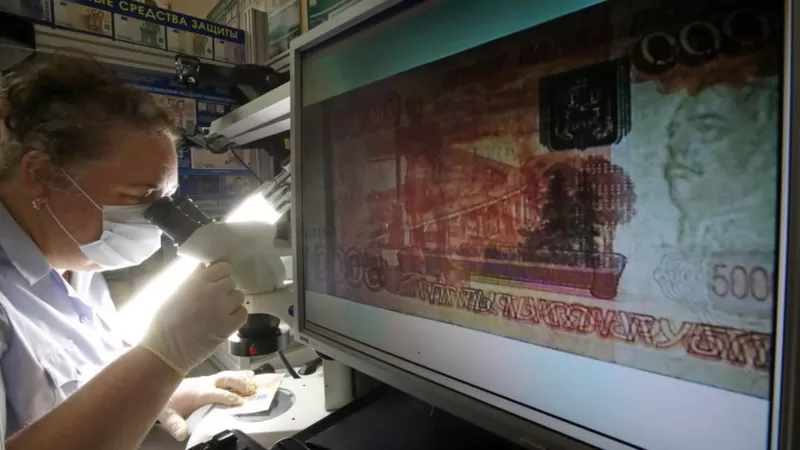
\includegraphics[width=0.58\textwidth]{img/bigmoney.png}
    \end{center}
    \caption{Благодаря грантам российские ученые могут получать конкурентные зарплаты, но других проблем государственные инициативы не решают.}
\end{wrapfigure}
Тогда же появились различные федеральные \explain{целевые}{target} программы, министерские \explain{конкурсы}{contests}. И к 2010 году, во время президентства Дмитрий Медведева, правительство учредило конкурс научных мегагрантов, рассчитывая привлечь \explain{ведущих}{leading} ученых в российские вузы.

Конкурс мегагрантов в основном создавался для поддержки \explainDetail{дорогостоящих}{дорогостоящий}{costly} исследований в стратегических направлениях науки, которые определялись \explainDetail{чиновниками}{чиновник}{official, officer}.

Так в стране \explain{укрепилась}{was strengthened} грантовая система финансирования научных исследований. \explainDetail{В отличие}{в отличие от}{unlike}, например, от американской грантовой системы, в которой деньги идут не на зарплаты ученым, а на проведение исследования, российские специалисты могли значительно улучшить собственное финансовое положение.

Попросивший не называть своего имени российский ученый, работающий в крупной московской лаборатории, рассказал: «На Западе сложно получить \explainDetail{постоянную позицию}{постоянная позиция}{permanent position} в университете, но если получил --- зарплата \explain{приличная}{decent}. У нас гораздо легче получить позицию, в образовательных учреждениях есть маленькая базовая зарплата, но это очень небольшие деньги, и жить на них \explain{затруднительно}{cumbersome, hard, straitened or awkward}, особенно в Москве».

\explainDetail{Вопрос}{вопрос}{issue, matter} зарплат в России решается \explain{исходя из}{based on} возможностей конкретного университета или \explain{НИИ}{научно-исследовательский институт}. Например, один из сотрудников подмосковного НИИ рассказал, что в последние годы начал получать \explain{надбавки}{allowances, perks} за публикацию научных статей в хороших журналах.

«С грантов мы можем получать нормальную зарплату, иногда даже больше, чем в Европе, но по большинству из них мы даже компьютер не можем купить, потому что деньги требуют тратить только на \explain{непосредственные}{immediate} нужды исследования по проекту», --- говорит ученый.

В России старший научный сотрудник получает в среднем 26 тысяч рублей (примерно 350 долларов), а профессор --- 36 тысяч в месяц.

По указу Владимира Путина, зарплата научных работников должна быть доведена до 200\% от средней по региону. Однако никакого дополнительного финансирования на достижение этой цели выделено не было. Чтобы достичь определенных президентом показателей, университеты начали переводить научных работников на половину \explainDetail{ставки}{ставка}{rate}.

Об этом впервые публично рассказала кандидат биологических наук из Института цитологии и генетики РАН Анастасия Проскурина. Во время встречи с Путиным она заявила, что вместо \explain{положенных}{due} 79 тысяч получает 25, а руководство института вместо повышения зарплат предложило ей перейти на \explain{полставки}{part-time}.


\subsection{Мыши в кармане}

Инвестиции в экспериментальное оборудование часто происходят \explain{без учёта того}{without taking into account}, где и как это оборудование будет установлено, потому что деньги выделяются на конкретные проекты.

\begin{wrapfigure}{l}{0.45\textwidth}
    \begin{center}
        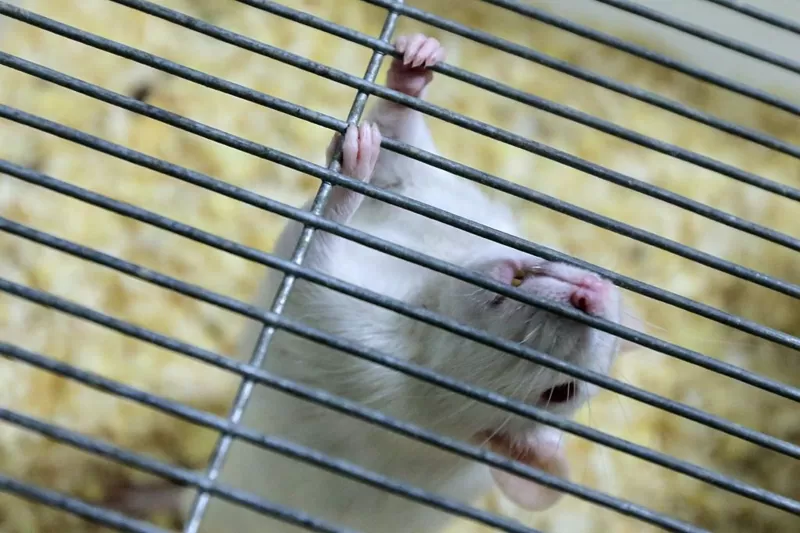
\includegraphics[width=0.44\textwidth]{img/mouse.png}
    \end{center}
    \caption{Процесс закупок трансгенных мышей из-за границы не был очевиден ни сотрудникам лаборатории, ни руководству университета.}
\end{wrapfigure}
«Мы покупаем \explain{сравнительно}{relatively} дорогостоящее оборудование, но во время ливней или \explain{таяния}{melting} снега на него начинает \explain{течь}{flow} вода, потому что университет годами не может нормально залатать крышу. \explainDetail{Оснащение}{оснащение}{equipment} образовательных лабораторий, где студенты проходят практикум, \explain{несравнимо}{incomparable} с западными», --- поделился на условиях анонимности сотрудник крупной московской лаборатории.

Одни лаборатории, созданные на деньги мегагрантов, успешно существуют до сих пор, а некоторые, даже после полного оснащения, закрываются без дальнейшей финансовой поддержки.

В 2011 году нейробиолог Виктория Коржова закончила Санкт-Петербургский государственный университет и работала в лаборатории, которая тоже создавалась на деньги мегагранта.


"С одной сторон\'{ы}, очень хорошее финансирование, а с другой --- денег недостаточно. Все время, которое грант действовал, ушло на организацию самой лаборатории, ремонт помещений и закупку оборудования", --- рассказывает Коржова.

Но для исследовательской работы не всегда достаточно просто оборудовать рабочие места.

В лаборатории, где работала Коржова, например, должны были проводиться эксперименты на трансгенных мышах. «Большинств\'{о} трансгенных мышей производит одна международная компания, которая \explain{поставляет}{supplies} их в лаборатории по всему миру, --- рассказывает она. --- Наш \explain{заведующий}{manager} лабораторией, у которого были деньги на закупку, не знал, как именно привезти мышей в Россию, каков легальный процесс. Университет тоже не мог ему помочь. В какой-то момент мы уже, не совсем \explain{шутя}{jokingly}, обсуждали, сможем ли мы привезти их в кармане, что совершенно безумная идея».

Проблема решалась почти два года. Все это время ученые были \explain{вынуждены}{forced} придумывать компромиссные варианты, чтобы, как они говорят, получилось что-то похожее на \explainDetail{первоначальную}{первоначальная}{initial, original} \explainDetail{задумку}{зад\'{у}мка}{idea, plan}.

Одна из важных проблем в России, которая давно решена в странах, где активно развивается наука, --- это отсутствие \explainDetail{таможенных}{таможенный}{related to customs ($<$ там\'{о}жня: customs)} \explainDetail{льгот}{льг\'{о}та}{privilege, benefit, exemption, discount} для научных закупок, считает нейробиолог.

В других лабораториях страны ситуация иная.

«Нет такой страны, которая бы производила все нужные реактивы для ученых. Нормально, что некоторые реактивы покупаются в США или Европе. При этом везде есть способ быстро получить \explain{доставку}{доставка}{delivery}, --- рассказывает Коржова. --- Работая в Германии, я могла \explain{заказать}{to order} антитела и получить их максимум в течение недели, а обычно --- за два-три дня».

В России же, по ее словам, люди ждут месяцами.

«Антитела --- очень \explain{чувствительные}{sensitive} вещества, которые нужно обязательно хранить в холоде. А если процесс на таможне \explain{затягивается}{drags on}, то неизвестно, как они хранятся. Из-за этого еще и эксперименты нужно планировать на год вперед, что не очень реалистично. Приходится идти на компромиссы: я делаю не так, как мне хотелось бы сделать в идеале, а существую в рамках больших ограничений», --- говорит нейробиолог.

\subsection{Возвращаются единицы}

Российский кристаллограф, член Европейской академии наук Артем Оганов уехал из России в 1997 году.

Он так вспоминает об этом: "Когда я уезжал, это был 1998 год, зарплаты были, ну я не знаю, пятьдесят долларов в месяц. Это нереально было для существования. Доктора наук продавали стиральный порошок на улице. Я решил уехать. Сейчас времена изменились".


В конце 2014 года Оганов, работавший в США, отказался от гринкарты и вернулся в Россию. "Если при прочих равных выбор: жить у себя дома или не у себя дома (вот я могу здесь заниматься передовой наукой и здесь, я могу и здесь иметь нормальный уровень жизни, и здесь), так вот выбирать нужно всегда свой дом", - объяснял он.

\begin{wrapfigure}{l}{0.5\textwidth}
    \begin{center}
        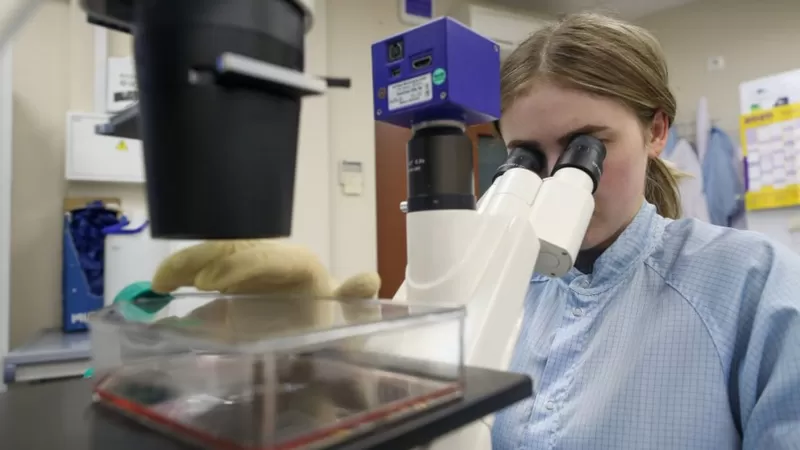
\includegraphics[width=0.48\textwidth]{img/microscope.png}
    \end{center}
    \caption{В России ученым не хватает свободы, считают некоторые уехавшие за границу.}
\end{wrapfigure}
"Таких, кто полностью вернулся в Россию, прервав основные контракты за рубежом, единицы. Подавляющее большинств\'{о} наших соотечественников, которые успешно работают за рубежом, свои позиции в научно-образовательных организациях развитых стран не оставляют, - говорит Сергей Ерофеев, работающий в американском университете Ратгерс. - Они прекрасно понимают, что это их основная жизнь. Если есть возможность успешно работать с коллегами в России, получать какие-то новые возможности для исследований - они иногда ухватываются за эту возможность".

Многие действительно стараются сохранять и использовать профессиональные связи в России.


Директор Центра нелинейной физики в Австралийском университете Юрий Кившарь был одним из первых получателей мегагранта. "Мы создали лабораторию - там было человек пять, потом она выросла в центр. Начали набирать новых людей, стало человек сорок. А потом центр стал кафедрой, а кафедра - факультетом. Так появился Новый физтех - физико-технический факультет университета ИТМО", -рассказывает Кившарь.

Сам ученый уехал в Австралию еще из СССР, но связи с российскими коллегами сохранил.

"Когда мы уезжали, это было другое время, - уверен он. - Многие толковые ребята уезжали, лишь бы уехать. Это был отъезд если не насовсем, то надолго. Сейчас у меня есть студенты из Москвы, и в основном они говорят, что уехали на время. Они не собираются оставаться. Сейчас вообще появилось больше возможностей поехать куда-то. В том же ИТМО молодежь посылают за границу на стажировку на год-два, но многие возвращаются", - говорит Кившарь.

\subsection{Национальная идентичность и воздух свободы}

Аспирант астрофизического факультета Принстонского университета США Айк Акопян, до этого работавший на кафедре физики и астрофизики МФТИ, вспоминает, как российские друзья прислали ему ссылку на статью с заголовком: "Американские ученые [далее шли типичные российские имена и фамилии] открыли…"

"Все трое, естественно, работали в США. Вообще сравнивать объем американской и российской науки невозможно, - рассказывает Акопян. - Здесь к науке относятся как к части культуры, как к национальной идентичности. Из-за этого есть частное финансирование науки - то, чего практически нигде в мире нет".

Акопян согласен, что в последние годы ситуация с финансированием науки в России начала улучшаться: "Я учился в России с 2010 года и уехал в 2016-м. За это время ситуация поменялась в лучшую сторону. Многие ученые начали получать огромное количество денег. Но финансы - не основная проблема".

Развития карьеры вне США, где в сфере астрофизики гранты на исследование выдает в том числе и NASA, Акопян не видит. Одним из основных достоинств он считает постоянное взаимодействие ученых.


\begin{wrapfigure}{l}{0.5\textwidth}
    \begin{center}
        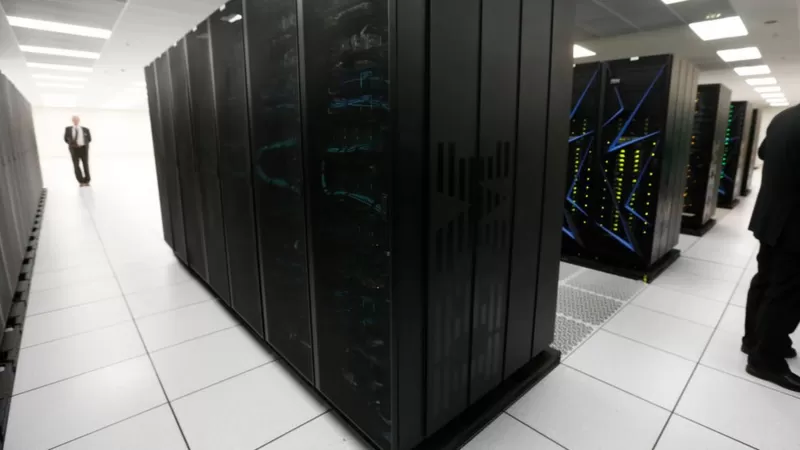
\includegraphics[width=0.48\textwidth]{img/supercomputer.png}
    \end{center}
    \caption{Российские ученые, уехавшие работать в США, считают, что возможностей для развития карьеры здесь больше, а научным сотрудникам доступно более современное оборудование. На фото - суперкомпьютер, на пользование которым можно получить отдельный грант.}
\end{wrapfigure}
"Когда открыли гравитационные волны, на следующий же день у нас была информация из первых рук: приехали ученые, которые рассказывали обо всех деталях открытия. Нам не приходится ждать всяких пресс-релизов, все становится открытым, ведется обсуждение. Когда миссия "Кассини" давала результаты - мы опять же всё узнавали от тех, кто занимался проектом".

Другой научный сотрудник университета США, переехавший за границу после окончания МФТИ, соглашается, что для нормальной работы ученых необходимо сочетание независимости и включенности в деятельность научного сообщества:


"Первое выражается в стабильной зарплате и возможности выбирать направления работы в широких рамках. Второе - в доступности участия в конференциях, семинарах, командировках. До сих пор один из важнейших критериев оценки ученых в Европе и США - это их репутация в международном научном сообществе. Обычно это дает гораздо более точное представление, чем формальные показатели".

"Самое главное, чего не хватает отечественным ученым, - воздуха. Того, что называется научной свободой. Страх сейчас проникает во все поры научного тела", - считает профессор Сергей Ерофеев.

С одной стороны, говорит он, руководство считает, что надо добиваться конкурентоспособности российской науки. Но есть и другая рука, которая главной своей задачей считает контроль.

"А контроль над обществом не предполагает свободы - даже научного мнения", - убежден ученый.

В 2018 году наука в России была официально объявлена национальным проектом. Нацпроект был разработан по следам майских указов Владимира Путина. Было обещано, что к 2024 году Россия должна войти в пятерку ведущих стран, осуществляющих научные исследования и разработки в областях, определяемых приоритетами научно-технологического развития.

Чиновники \explain{по-прежнему}{still} обещают создать \explain{привлекательные}{attractive} условия для работы ведущих российских и зарубежных ученых, а также увеличить финансирование научных проектов и разработок.




\section{Война на Украйне}
\subsection{Запад не поверил предупреждениям Владимира Путина}
% https://russian.rt.com/inotv/2022-02-28/AC-Zapad-ne-poveril-preduprezhdeniyam

Многие считают Владимира Путина нерациональным, однако российский президент сделал именно то, о чём \explainDetail{предупреждал}{предупреждать/предупредить}{warn, let know beforehand}, и специальная военная операция на Украине является ответом на \explain{отказ}{refusal} от расширения НАТО, считает американский политик и публицист, главный редактор журнала The American Conservative Патрик Бьюкенен. По его мнению, Путин не хочет войны с Западом, однако для этого Байдену нужно \explain{пересмотреть}{rethink, revise} своё видение Североатлантического альянса.

Когда Владимир Путин потребовал, чтобы США исключили Украину из числа будущих членов альянса НАТО, США ответили, что НАТО проводит политику «открытых дверей» и любая страна, включая Украину, может \explain{подать заявку}{apply, submit application} на членство и быть принятой в альянс. Как считает американский политик и публицист, главный редактор журнала The American Conservative Патрик Бьюкенен, не \explainDetail{сум\'{е}в}{ум\'{е}ть/сум\'{е}ть}{to be able, to manage, to succeed} получить \explain{удовлетворительный}{satisfactory} ответ на своё требование, Путин сделал именно то, о чём он предупреждал, и начал специальную военную операцию на Украине.
Как продолжает Бьюкенен, каким бы ни был характер российского президента, он подтвердил одно: ему можно верить, и когда Путин предупреждает, что он что-то сделает, он следует своим словам. И теперь Западу стоит ответить на два вопроса: как он дошёл до этого и куда теперь двигаться дальше?

\begin{fancyquotes}
    «Как мы дошли до такого положения, когда Россия, оказалась \explainDetail{прижатой}{приж\'{а}тый, -ая (прижать)}{to press} \explainDetail{спиной к стене}{прижатый спиной к стене}{with one's back against the wall}, а Соединенные Штаты, пододвигая НАТО все ближе к границам России, ещё больше загон\'{я}ли её в угол?», --- пишет Бьюкенен.
\end{fancyquotes}

Для этого автор статьи \explain{призывает}{calls} посмотреть в прошлое. В период с 1989-го по 1991 год Михаил Горбачёв позволил \explain{снести}{tear down} Берлинскую стену, \explain{воссоединить}{reunit} Германию и освободить все «\explain{порабощённые народы}{enslaved nations/people}» Восточной Европы. Также Горбачёв позволил Советскому Союзу \explain{распасться}{fall apart} на 15 независимых государств, \explain{отменил}{cancelled, abolished, put an end to} холодную войну в Европе, \explainDetail{устранив}{устран\'{и}ть}{eliminate} со стороны Москвы все причины для исторического \explainDetail{раскола}{раскол}{schism, split} мира.

Путин \explain{пришёл к власти}{came to power} в 1999 году после «катастрофического десятилетнего правления Бориса Ельцина, который \explain{букв\'{а}льно}{literally} \explain{втоптал}{trampled} Россию в землю». В том же 1999 году Путин \explain{наблюдал}{observed, watched, oversaw}, как Америка провела 78-дневную кампанию бомбардировок Сербии. В том же году три бывшие страны Варшавского договора: Чехия, Венгрия и Польша --- были приняты в НАТО.

\begin{fancyquotes}
    «Тогда \explain{справедливо}{righteously} \explain{возник}{past tense of возн\'{и}кнуть (arise)} вопрос: от кого эти страны должны были быть защищен\'{ы} американским оружием и альянсом НАТО?» --- пишет Бьюкенен.
\end{fancyquotes}

По его мнению, прямой ответ на этот вопрос был дан в 2004 году, когда Словения, Словакия, Литва, Латвия, Эстония, Румыния и Болгария были приняты в НАТО. Затем, в 2008 году, была принята Бухарестская декларация, которая поставила Грузию и Украину, граничащие с Россией, в очередь на членство в НАТО.

В том же году Грузия \explain{напала}{attacked} на Южную Осетию, что спровоцировало Россию на ответ. Американский \explain{истеблишмент}{establishment} объявил, что это была агрессивная война России, но впоследствии проведённое Евросоюзом расследование \explain{обвинило}{accused} в развязывании войны президента Грузии Михаила Саакашвили.

А потом, пишет Бьюкенен, был Крым. В 2014 году демократически избранный президент Украины Виктор Янукович был \explain{свергнут}{overthrown} в Киеве и \explain{заменён}{replaced} прозападным режимом. \explain{Вместо того чтобы}{instead of} потерять Севастополь, историческую военно-морскую базу России в Крыму, Путин \explainDetail{присоединил}{присоедин\'{я}ть/присоедин\'{и}ть}{to join, to link, to add, to connect, to attach; here: to annex}* полуостров к России. И всё это, пишет Патрик Бьюкенен, подводит нас к сегодняшнему дню.

\begin{fancyquotes}
    «\explain{Что бы мы ни думали о Путине}{whatever we think about Putin}, он --- не Сталин. Он не убивал миллионы людей и не создавал архипелаг ГУЛАГ. Он не нерационален, в чём \explainDetail{обвиняют}{обвин\'{я}ть/обвин\'{и}ть}{accuse} его некоторые учёные мужи. Он не хочет с нами войны, которая была бы более чем \explain{разрушительной}{destructive} для обеих сторон. Путин --- русский патриот, традиционалист, холодный и \explain{безжалостный}{ruthless} реалист, \explain{стремящийся}{aspiring} сохранить Россию как великую и уважаемую \explainDetail{державу}{держава}{power}, которой она когда-то была. И он верит, что она может снова стать такой», --- пишет Бьюкенен.
\end{fancyquotes}

Однако этого не может произойти, если расширение НАТО не \explainDetail{прекратится}{прекращ\'{а}ться/прекрат\'{и}ться}{stop} или если родственное России государство Украина станет частью военного альянса, который больше всего гордится тем, что выиграл холодную войну против страны, которой Путин служил всю свою жизнь.

\begin{fancyquotes}
    «Президент Джо Байден почти ежечасно обещает: «Мы не собираемся воевать на Украине». Почему же тогда он не готов исключить членство Украины в НАТО, которое потребовало бы от нас того, что, по слов\'{а}м самог\'{о} Байдена, мы, американцы, никогда не должны делать ради нашего же собственного выживания: начать войну с Россией», --- пишет главный редактор The American Conservative.
\end{fancyquotes}

\textit{*Крым вошёл в состав России после того, как за это \explainDetail{проголосовало}{голосов\'{а}ть/проголосов\'{а}ть}{to vote} подавляющее большинств\'{о} жителей полуострова на референдуме 16 марта 2014 года (прим. ИноТВ).}




\subsection{Ставки продолжают повышаться}
% https://novayagazeta.ru/articles/2022/02/27/stavki-prodolzhaiut-povyshatsia

\textit{В кризисе вокруг Украины теперь напомнили о ядерных силах России}

Президент РФ Владимир Путин приказал привести российские силы \explainDetail{сд\'{е}рживания}{сд\'{е}рживание}{containment} в режим особого несения \explainDetail{дежурства}{дежурство}{duty}. Это демонстративное действие для \explain{св\'{е}дения}{intelligence (used in plural)} стран НАТО произошло в воскресенье во время встречи с министром \ed{обороны}{министр обороны}{minister of defence} Сергеем Шойгу и начальником Генштаба Валерием Герасимовым.

На памяти опрошенных нами ветеранов такой случай были лишь однажды --- в момент операции по \ed{присоединению}{присоединение}{annexation} Крыма, об этом президент Путин сам рассказал ВВС. В советское время такое происходило дважды в 1962 и 1983 годах. Однако \ed{подтверждений}{подтверждение}{confirmation} из других \ed{источников}{источник}{source}, что силы ядерного сдерживания были переведены в особый режим весной 2014 пока нет.

Основы госполитики в сфере ядерного сдерживания Путин \explain{утвердил}{approved} в июне 2020 года. Согласно этому указу все ключевые решения, в том числе о переводе сил сдерживания в особый режим, принимает лично он. Причин, по которым вводится такой режим, несколько, и все они связываются с подготовкой других стран к применению против нашей страны ядерного оружия.

Однако, есть там и такое \explain{условие}{condition} перехода на особый режим, которое \explain{соответствует}{corresponds} нынешней ситуации на Украине, после начала там спецоперации ВС РФ.

\begin{fancyquotes}
    «Развертывание государствами, которые рассматривают РФ в качестве потенциального противника, систем и средств противоракетной обороны, крылатых и баллистических ракет средней и меньшей дальности, высокоточного неядерного и гиперзвукового оружия, ударных беспилотных летательных аппаратов, оружия направленной энергии» --- о таких шагах президент России говорил в своих речах неоднократно.
\end{fancyquotes}

Говоря языком военной разведки, перевод стратегических ядерных сил (СЯС) на особый режим осуществляется при вскрытии мероприятий противника по подготовке своих ядерных сил, а предотвратить кризис другим способом невозможно. Угроза разгрома ключевой для обороноспособности страны группировки войск также может привести к ответной угрозе применения ядерного оружия со стороны России. В этих случаях речь идет о вероятном нанесении ударов тактическим ядерным оружием.

Пока неизвестно, как ведут себя (и ведут ли как-то вообще) авианосные ударные группировки США, перебазировались ли стратегические бомбардировщики на аэродромы Англии и Италии, откуда они обычно летали в Ирак. Также не поступало информации о какой-то угрозе, нависшей над группировкой ВС РФ на Украине.

Скорее всего, перевод СЯС на особый режим является превентивной мерой в адрес стран НАТО, публичным предостережением от участия в военных действиях на стороне ВСУ. Тем более, что, по словам опрошенных нами авторитетных специалистов по стратегическим вооружениям, российские силы сдерживания всегда и постоянно находятся в состоянии полной готовности. Безо всяких об этом объявлений.

\subsection{«Никто не хочет к вам»}
\textit{Монолог IT-архитектора Андрея Ключко, четвертый день сидящего в подвале частного дома в Харькове}

Я нахожусь в Харькове, в северной части города, в доме моих родителей, в частном секторе. Все это время с 5 утра [24 февраля], когда начали ******* [бомбить], мы сидим в подвале. Первую ночь тут была вся семья, все собаки, и даже тетка приходила. Утром второго дня всех, кого можно было поместить в одну машину --- трех женщин, трех собак и трех котов --- мы отправили во Львов. Они уже там, но очень много людей едет, большие не пробки, но «тягучки»: на блокпостах их проверяют и отпускают. Кто остается во Львове, кто-то едет в Карпаты, кто-то в Польшу, там на границе большие очереди.

Сегодня [27 февраля] четвертый день, в районе 8-9 утра заехали [в город] ваши ребятки просто на джипах БМП, и следующие два часа их тут били и жгли --- есть куча видео в телеграм-каналах. Все это сопровождается периодическими арт-обстрелами. То мы стреляем, а те отвечает, то те стреляют, а мы тут жухаемся. В городе много всего разбомбленного.

\textbf{Было ли страшно.}
Страха толком не было. Первые пару минут обстрела, когда было темно и вообще ни хрена непонятно, что происходит и кто где. Когда начинаешь понимать диспозицию сил, что происходит вокруг, какой тип оружия стреляет, что он может, чем больше ты понимаешь в боевых действиях, тем спокойнее их воспринимать.

\textbf{Как устроена жизнь}
У нас с отцом в подвале житейские условия плюс-минус хорошие. У нас и свет, газ и вода. В наличии еда, но есть сейчас как-то не хочется. До вчерашнего дня даже был wi-fi, но вчера обстреливали очень сильно Салтовку (знаменитый район Харькова, крупнейший жилмассив бывшего СССР --- прим. «Новой»), и много, где пропал свет. У нас он остался, но у провайдера --- нет, поэтому wi-fi больше нет, хотя я его успел в подвал провести.

Приходится ловить мобильный интернет, а для этого вылезать из подвала, а это небольшой стресс, поскольку очень много шума и стрельбы вокруг, и ничего непонятно. У нас дом расположен на возвышенности, а это частный сектор, и тут толком ничего нет, поэтому ночью хорошо слышно все вокруг, и кажется, что снаряды бьют прямо сюда. Но психологически мы к этому уже привыкли, просто надо сидеть и ждать. Хорошо, что есть хотя какая-то связь, вообще без нее было бы тяжело. А так видишь, что

\begin{fancyquotes}
    у нас есть военные успехи, и мораль на очень высоком уровне. У всех, кого я знаю.
\end{fancyquotes}

Большинство знакомых поуезжали или поотправляли своих на запад. Те, кто живут в жилмассивах, стараются сидеть в подвалах, куда-то закапываться. На Салтовке уже довольно много взорванных подъездов --- на улице Бучмы сегодня точно был взорван дом напротив заправки, но надеюсь, людей там уже не было.

Я живу довольно далеко от центра, до ближайшей станции метро километров 5-6, и мы, конечно, туда не ходим. А те, кто в центре или ближе к метро, спускаются туда. Никакого гуманитарного ужаса в плане отсутствия еды и воды нет. Магазины закрыты, но в метро привозят еду, а те, кто сидят по подвалам, закупились в первый день.

\textbf{Как узнавать информацию.}
Мы сидим все в харьковских чатах, и когда слышим какие-то «прилеты» или «отлеты» ракет, то сверяем по чату. Раньше это было сообщество где-то сотни людей, которые играют в квесты, а теперь мы это чат харьковской переклички, люди по разным районам контролируют кто, что и где.

\begin{fancyquotes}
    Слухов особенно нет, да и я стараюсь не читать ничего, что похоже на «кум моего знакомого парня из СБУ сказал».
\end{fancyquotes}

Читаю официальные каналы, УНИАН и «Суспильное», и этого в принципе хватает для понимания. Большинство сообщений в этих каналах обнадеживающие и поддерживающие, поэтому настроение довольно высокое.

\textbf{Почему не уехал.}
Я с самого начала знал, что я никуда не поеду. Сложно это объяснить, но для меня даже вопрос такой не стоял. Я в принципе знал, что у родителей есть подвал, хотя никто в семье до последнего момента об этом не упоминал. И готовили [для жизни] мы его уже во время первого обстрела утром первого дня.

Но я знал, что даже если будет самый плохой сценарий --- какой примерно и произошло --- это дает какое-то [ощущение] тыла. Люди без такого тыла и понимания, что делать, больше боялись и больше были склонны переехать ближе к западной границе. Сыграло свою роль и то, что в моей семье много родственников живут в «ДНР» и «ЛНР». Они передали мне опыт сидения под обстрелами, распознавания разных видов вооружения. Мы все знали, что это часть жизни --- но раньше это была часть жизни наших родственников, а теперь и нашей. И это не так страшно, но тем, кто так близко не соприкасался --- а у меня мама и папа родом с территории Донецкой и Луганской областей, ныне контролируемой «ДНР» и «ЛНР» --- наверное, было сложнее справляться со стрессом.

\textbf{Отношение к происходящему.} Честно? Спокойное. Просто хочется, чтобы это закончилось и дошло до нашей логической победы. Нам сейчас нужно воевать, в переговоры верится слабо. Я не понимаю, какие гарантии Россия может дать кому-либо, даже своим гражданам. У многих ощущение, что чем больше украинские вооруженные силы нанесут ущерба российским вооруженным силам, тем ближе конец этого всего, и это единственный путь. Но лично меня деморализовали подвижки нашего украинского руководства к каким-то переговорам. Это мое личное отношение.



\textbf{Жертвы среди мирного населения.} Они есть, но надо сказать, что когда мы видим попадания в девятиэтажки, что в Киеве, что на Салтовке, то эти дома, слава богу, по крайней мере частично были «самоэвакуированы». В каналах выкладывают информацию о погибших людях, но с большинством из них это случилось на улице. Это те, кто не успел добежать до бомбоубежища или по какой-то причине не пошел туда.

Есть такая ироничная точка зрения, что харьковчанам несколько все равно на происходящее. Из забавного я видел просьбу от наших официальных сил не ждать транспорта в связи с военной ситуацией. Я просто представил, что где-то сейчас стоят люди на остановках и ждут трамвая. Или вот мой приятель с Салтовки ответил на мой вопрос о том, как у него дела, так: «Да все в порядке, обычная салтовская история. Грабят магазины, бьем тех, кто грабит… Ну да, еще бомбят». Жертвы единичны или, возможно, их десятки, но как оценить не знаю. Про жертвы среди военных информации почти нет.

\textbf{Верилось ли, что может быть война?}
Я долгое время игнорировал [разговоры о будущей войне], потому что эта новостная тревога девальвируется. Путин что-то сказал, Песков что-то сказал, и я начал на всех злиться: «Путин, ну сколько можно, Байден, перестань, это просто какая-то херня». И я очень злился на все медиа --- и украинские, и российские, потому что каждый чей-то вздох превращался в [алармистские] заголовки. Я думал, зачем нужен этот пустой звон, и хотелось сказать: «Заткнитесь все, ведь если что-то произойдет, мы узнаем первые». Потом люди начали куда-то собираться, совершенно случайно --- в давно запланированные командировки и отпуска, начали покидать страну. Я понимаю, почему, но это немного раздражало. Я долгое время хранил скептически-саркастический взгляд: «Ну да, ну едьте, ну и сидите там». 90\% людей, которые сейчас находятся во Львове, выехали туда уже во время боевых действий, это все решается, и незачем было развивать эту панику до начала событий.

Я ожидал какого-то адища по линии соприкосновения «ДНР», «ЛНР» и Украины, но что начнут Харьков, Одессу, Херсон и Киев херачить --- нет. Около «ДНР» и «ЛНР» стояли наши лучшие части, самые опытные, и они сильно зашиты в землю, они копали окопы все эти 8 лет, и я думал, что их оборону просто не прорвут. И все эти Совбезы, разрешения Совфеда [на ведение войны] меня не волновали, потому что я знал, что у нас есть армия, и если что, мы будем драться. То, что сейчас делал Путин, мы видели и перед Крымом. Ощущение было такое: «Ну да, и что? Так это уже было. Пусть входит --- будем воевать». Слава богу, что мы не струсили, мы стоим, и у нас есть армия. Это круто видеть, что она вооружена и профессиональна, и это не какие-то солдатики в советских кирзовых сапогах, как было в 2014 году.


\textbf{Почему так мало эмоций} Есть заезженная фраза, что война идет уже 8 лет. И, действительно, если бы я записывал это аудиосообщение в 2014 году, то я бы, наверное, срывался на более высокие ноты. Сейчас, после всего, что произошло с моими родственниками на Донбассе, мы не то, что привыкли, но психика адаптировалась к этому агрессору, и ты воспринимаешь эту ситуацию более спокойно. Нет смысла что-то орать, махать кулаками и психовать. Отношение --- крайне агрессивное и негативное, но оно уже так долго такое, что выражать его наружу, наверное, психика уже устала. Надо просто воевать и закончить с этим всем.

Но я могу сказать, что все, кто причастен к этой войне со стороны РФ, --- мрази и ублюдки. Если они все умрут, я буду крайне счастлив, а все, что происходит здесь --- это полный ******* [кошмар]. И одно дело защищать какие-то принципы, даже выдуманных нацистов на Донбассе бить, но

\begin{fancyquotes}
    кого вы бьете в Одессе, Киеве и Харькове? Каких нацистов? Это просто полный сюр!
\end{fancyquotes}

\textbf{Что, если Харьков оккупируют?}
Город не будет оккупирован ни в коем случае, судя по тому, что я вижу, грубо говоря, из окна. Сегодня, когда утром заезжали российские боевые машины с севера и ехали куда-то на скорости, это увидели все. Ведь до этого [происходило] по сути, на окраинах, а сегодня какие-то машины доезжали чуть ли не до центра, где их уничтожали. Было такое впечатление, что они ехали просто бесцельно, и это приводит в замешательство. Очевидно, что большие города-миллионники не захватываются сотней другой боевых машин, это делается не так, и непонятно, зачем это кому-то было нужно.

Чтобы оккупировать Харьков, нужно выбить отсюда украинские войска авиаударами --- этого нет, потом заходить колоннами танков --- этого тоже нет. И остаются люди, Харьков --- полуторамилионный город, и людей здесь до сих пор до хрена. Это огромный город, нелояльный россиянам. Большая разница с Донецком в 2014 году, который был лоялен россиянам. Тогда люди из Донецка видели Крым, у них был пример, они хотели к вам, в Россию. Сейчас в Харькове все видели, что происходит эти 8 лет в «ДНР» и «ЛНР», весь этот ****** [ужас], людей, ездящих за пенсией к нам.

\begin{fancyquotes}
    Никто не хочет к вам. Что вы будете делать с этими людьми?
\end{fancyquotes}

Вырезать и убивать, а потом перевозить сюда из Донецка людей, которые должны будут стать харьковчанами? В этот бред не верится. Абсурдность всего того, что я сейчас произнес, говорит о том, что этого не произойдет. Но даже если бы нас тут сравнивали просто с землей, то я бы все равно оставался в подвале. Я бы не бежал никуда. Я бы просто ждал. Не знаю чего.

Мне трудно ответить на такой вопрос, потому что я вообще об этом не думал. Это как спросить: «Андрей, что ты будешь делать, если окажешься в марсианской экспедиции?» От меня это столь же далекая перспектива, как и оккупированный Харьков. И это касается практически каждого областного центра --- я не верю, что они будет оккупированы и заняты, и даже вроде как занятый российской армией Херсон, уверен, будет освобожден в ближайшие дни.

\textbf{Обращение к обычным россиянам.} Я ничего не хочу сказать обычным россиянам, среди которых много моих знакомых. Мне кажется, они сами все знают.

В отборе на Евро-2000 Андрей Шевченко в Лужниках в стыковом матче забил знаменитый гол Филимонову за шиворот. Мне было примерно 10-11 лет, и я плакал у телевизора и был счастлив (кажется по голосу, что Ключко и сейчас начинает плакать --- прим. «Новой»). И я ничего не хотел сказать обычным российским болельщикам, мне было на них все равно. Я хотел сказать тогда украинским болельщикам и сейчас --- украинским гражданам, что мы ******** [классные] и мы победим.

\subsection{Кремль ответил на вопрос о возможном столкновении России и НАТО}
% https://lenta.ru/news/2022/02/28/kremlind/
\textit{Песков счел неприемлемыми высказывания о возможности прямого столкновения России и НАТО}

Любые высказывания о возможности прямого столкновения России и НАТО неприемлемы, заявил официальный представитель Кремля Дмитрий Песков, комментируя соответствующий вопрос, сообщает ТАСС.

Решение российского президента Владимира Путина о переводе сил сдерживания на особый режим боевого дежурства последовало, в частности, после заявлений главы МИД Великобритании, отметил Песков.

«Были высказывания разных представителей на разных уровнях о возможных конфликтных ситуациях и даже коллизиях и столкновениях между НАТО и Россией», --- добавил представитель Кремля.

27 февраля Путин приказал начальнику Генштаба Вооруженных сил России Валерию Герасимову и главе Минобороны Сергею Шойгу перевести российские силы сдерживания в особый режим несения боевого дежурства.

24 февраля президент России Владимир Путин объявил, что принял решение о проведении специальной военной операции по защите Донбасса. Об этом он заявил во время обращения к гражданам.

\subsection{Начал\'{и}сь переговоры Украины и России}
% https://lenta.ru/news/2022/02/28/start/
\textit{В Белоруссии начал\'{и}сь переговоры делегаций из Украины и России}

В Белоруссии начал\'{и}сь переговоры делегаций из Украины и России, сообщает \explain{БЕЛТА}{Белорусское телеграфное агентство}.

Российскую делегацию возглавляет помощник президента, бывший министр культуры Владимир Мединский. С украинской стороны присутствуют министр обороны, глава фракции «Слуга народа» в Верховной Раде и замглавы МИД.

27 февраля пресс-секретарь президента России Дмитрий Песков заявил, что делегация из РФ прибыла в Гомель для переговоров и ждет украинских представителей. Президент Украины Владимир Зеленский сказал, что Киев готов вести переговоры в Варшаве, Братиславе, Будапеште, Стамбуле или Баку. «Да и любой другой город нам подходит. В стране, с территории которой не летят ракеты», --- пояснил он.

Позже стало известно, что переговоры пройдут на границе Украины и Белоруссии. Утром 28 февраля белорусский МИД сообщил, что площадка для встречи двух делегаций подготовлена.

\subsection{Российская авиация завоевала господство в воздухе над всей территорией Украины}
% https://lenta.ru/news/2022/02/28/minoborony/
\textit{Минобороны: боевая авиация РФ завоевала господство в воздухе над территорией Украины}

Боевая авиация России завоевала господство в воздухе над всей территорией Украины. Об этом «Ленте.ру» заявил официальный представитель министерства обороны страны генерал-майор Игорь Конашенков.

Он рассказал, что российские воздушно-космические силы за минувшие сутки уничтожили восемь боевых машин «Бук М-1», станции наведения ЗРК С-300 и «Бук М-1», а также три радиотехнические позиции со станциями П-14, четыре боевых самолета на земле и один в воздухе.

По словам Конашенкова, всего с начала операции уничтожено 314 танков и других бронированных машин, 57 реактивных систем залпового огня, 121 орудие полевой артиллерии и минометов, а также 274 единицы военной автомобильной техники.

Ранее официальный представитель ведомства сообщил, что украинцы, проживающие в Киеве, могут беспрепятственно покинуть город. Он напомнил, что российская военная операция не угрожает гражданскому населению. Основной целью Вооруженных сил (ВС) являются только военные объекты.

О начале военной операции по защите Донбасса стало известно 24 февраля, после обращения президента России Владимира Путина к населению. По его словам, к этому Москву вынудила сложная обстановка в Донецкой и Луганской народных республиках (ДНР и ЛНР).

\subsection{Перекрыли воздух}
% https://lenta.ru/articles/2022/02/28/avia/
\textit{Европа закрыла воздушное пространство для самолетов из России. Как это отразится на туристах?}

28 февраля Европа в ответ на спецоперацию в Донбассе полностью перекрыла воздушное пространство для самолетов, имеющих отношение к России. Кроме того, санкции Евросоюза сделали фактически невозможным использование зарубежных самолетов отечественными перевозчиками, а также спровоцировали проблемы с использованием банковских карт за рубежом. Последствия не заставили долго себя ждать: за границей снова оказались изолированы тысячи российских туристов, которые не знают, как вернуться домой и как закончится их отпуск. О том, чем обернулось обострение отношений между странами для авиаотрасли и туризма, --- в материале «Ленты.ру».

\textbf{Мир захлопнулся.}
Проблемы с перелетами у россиян начались еще 24 февраля, в первый день спецоперации в Донбассе --- несколько российских аэропортов в южных городах, включая Брянск, Сочи, Симферополь, Астрахань и Краснодар, отменили рейсы из-за близкого расположения к границе с Украиной, где началась военная операция. В результате, кто-то не смог вернуться домой с отечественных курортов, а другие --- застряли за границей, поскольку должны были прилетать в «закрывшиеся» хабы.

Позже для россиян оказалась закрыта и вся Европа. Одной из первых авиасообщение ограничила Великобритания. Вслед за ней Бельгия предложила ЕС запретить оформлять визы россиянам, а Литва и Чехия рассмотрели это как руководство к действию и незамедлительно прекратили выдачу въездных документов отечественным

\begin{center}
    \bf \Large Евросоюз запретил воздушным судам российских перевозчиков приземляться, взлетать или пролетать над территорией союза
\end{center}

После этого европейские страны одна за другой начали захлопывать свои воздушные пространства для российских перевозчиков, постепенно разрушая любые надежды на отпуск в ближайшее время. Среди них оказались Эстония, Франция, Германия, Норвегия, Латвия, Литва, Словения, Испания, Финляндия, Греция, Швеция, Италия, Португалия, даже миролюбивая Исландия и многие другие. В итоге решение поддержала почти вся Европа и Канада.

Таким образом, популярные курорты вроде Кубы, Мексики и Доминиканы оказались отрезаны для туристов, поскольку полеты в эти страны всегда проходили через Норвегию, Швецию и Латвию, и теперь изменение маршрутов сопряжено с колоссальным возрастанием цены на авиабилеты.

Как сообщает Ассоциация туроператоров России (АТОР), в системах бронирования компаний уже исчезли путевки в Доминикану, на Кубу, в Мексику и Венесуэлу на все даты. А в Azur Air пообещали, что оставшиеся на отдыхе туристы будут вывезены в соответствии с датами, указанными в турах. При этом, как сообщают туристы, вернувшиеся с Кубы 27 февраля, теперь перелет до Москвы занимает не 13 часов, как это было ранее, а 17.

\textbf{«Все упирается в деньги».} Заслуженный пилот России Юрий Сытник считает, что одним из способов решения возникшей проблемы может быть разработка новых полетных маршрутов. По его словам, самый короткий путь лежит через Северный Полюс по нейтральным водам --- таким образом, можно миновать Данию, Швецию, Финляндию и Норвегию через Мурманск. Однако самолетам все равно придется «подсаживаться» на каких-то островах для дозаправки, где еще открыто воздушное пространство.

\begin{fancyquotes}
    Второй маршрут --- через Азию. То есть через Израиль, Иран, затем через Баку или Казахстан. Все это можно сделать, но надо иметь в виду, что стоимость перевозки вырастет в два или три раза. Не все люди могут заплатить такие деньги

    \hfill\textit{заслуженный пилот России Юрий Сытник}
\end{fancyquotes}

Кроме того, поскольку туристы начали переживать, что полеты в Европу могут угрожать их безопасности, летчик заверил, что военные действия не представляет угрозы для пассажирских лайнеров. Эксперт также рассмотрел альтернативные варианты полета в европейские страны.

«Для россиян нет никакой опасности летать в Европу иностранными компаниями. Там войны нет, самолеты гражданской авиации стабильно летают. К тому же, правительство может договориться с китайскими, индийскими, арабскими перевозчиками. Варианты есть, но все упирается в деньги.

Над Турцией тоже можно летать спокойно. При хорошем управлении воздушным движением перегруза воздушного пространства быть не должно. Например, в ночные часы в Европе летает мало самолетов и воздушное пространство более менее свободно. Так что пройти на высоте 10-12 километров не составляет труда на большегрузных самолетах. Например, Boeing-747, Boeing-767, Boeing-777.

Нужно только поменять самолеты с вместимостью на 180-200 кресел на лайнеры вместимостью 400-500 кресел. Это необходимо, чтобы уменьшить количество воздушных судов одновременно в зонах управления движением, но при этом увеличить количество пассажиров в зоне перевозки на одном рейсе».

\textbf{Подрезали крылья.} Другой проблемой, которая взволновала всю авиаотрасль, является новый пакет санкций Евросоюза, а именно --- та часть, которая касается запрета на поставку европейских самолетов в Россию. Речь идет об авиалайнерах компании Airbus, которые составляют значительную часть российского авиапарка. Согласно данным Росавиации, всего отечественные перевозчики эксплуатируют 322 самолета Airbus. По подсчетам РБК, эти самолеты обеспечивали 40 процентов пассажиропотока в России.

\begin{center}
    {\bf \huge 322 самолета Airbus}

    \textbf{эксплуатируют российские компании на данный момент}
\end{center}

Фактически санкции ЕС лишают российские авиакомпании возможности использовать Airbus. При этом, как рассказал в беседе с «Ъ» эксперт Института экономики транспорта и транспортной политики НИУ ВШЭ Федор Борисов, самую большую угрозу представляет именно пункт о запрете техобслуживания и поставки запчастей.

«Запрет исключительно поставок и лизинга новых самолетов ближайшие несколько лет не стал бы критичным: в России достаточно большой и современный парк, который может эксплуатироваться продолжительное время без модернизации. Но в принятом виде глобальную угрозу представляет пункт о запрете техобслуживания и поставки запчастей и комплектующих для авиапроизводства», --- уточнил он и добавил, что ни одна страна в мире не производит всего комплекса деталей и механизмов, требующихся для создания самолета.

Кроме того, эксперт предположил, что если США примут аналогичные санкции, российский авиапарк может лишиться и самолетов Boeing --- их в России не менее 400.

Уже сейчас, по данным АТОР, несколько отечественных авиакомпаний столкнулись с проблемами за границей. Например, как сообщает Telegram-канал FrequentFlyers, Nordwind Airlines 27 февраля лишилась самолета в Мехико. Поскольку страховка Boeing 777-300ER была аннулирована из-за санкций, лайнер не смог вернуться в аэропорт вылета в Хабаровске.

В связи с этим, согласно прогнозам экспертов, в понедельник, 28 марта, ряд крупных российских авиакомпаний может объявить об отмене рейсов даже в открытые страны. Этому способствует не только опасение потерять самолеты, но также отсутствие возможности летать над Европой.


\textbf{Что делать?} Всех этих рисков, а также проблем с платежными системами за рубежом после санкций ЕС, оказалось достаточно, чтобы российские туристы сами расхотели лететь на отдых из-за страха застрять за границей без средств к существованию. Уже 25 февраля туроператоры сообщали о 40-процентном снижении продаж туров в иностранные государства.

Кроме того, в сложившихся обстоятельствах путешественникам стало психологически некомфортно думать об отдыхе и планировать отпуск на море даже на отечественных курортах. На это обратил внимание генеральный директор туроператора «Дельфин» Сергей Ромашкин. В разговоре с «Ъ» он подчеркнул, что продажи весенних туров на черноморские курорты России сократились на 50 процентов, а объем продаж летних путевок упал примерно на 35 процентов.

\begin{center}
    {\bf \huge 150 тысяч россиян}

    \textbf{находятся за границей в данный момент}
\end{center}

К тому же, в Ростуризме рекомендовали отказаться от поездок на юг России и за границу в ближайшее время. В ведомстве уточнили, что стоит рассмотреть перенос дат путевок или связаться с авиакомпаниями для выяснения актуальной информации по рейсам.

На данный момент, по оценке Аналитической службы АТОР, за рубежом находится около 150 тысяч российских путешественников, при этом более 27 тысяч из них могут испытывать проблемы с возвращением домой. Учитывая это, Ростуризм совместно с Росавиацией и МИД начали разрабатывать план по возвращению туристов. График рейсов будет сформирован после того, как ведомства получат информацию об объемах перевозок.

Сейчас тех, кто не может улететь из-за границы, просят держать связь с туроператорами и авиакомпаниями, а также в обязательном порядке зарегистрироваться в приложении «Зарубежный Помощник» МИД России (ссылка для скачивания iOS и Android).

\begin{center}
    \bf Также россияне могут сообщить о возникших проблемах на горячую круглосуточную линию МИД +7-(495)-695-45-45 или на горячую линию Ростуризма 8-(800)-200-34-11 (с 8:00 до 20:00 по московскому времени)
\end{center}

\textbf{Выход есть.} Россияне, которым необходимо улететь за границу, все еще могут воспользоваться услугами зарубежных авиаперевозчиков, а также выбрать стыковочные рейсы через Турцию для поездок в Европу. Безусловно, это увеличивает время полета и стоимость перевозки, но в случаях крайней необходимости сейчас это самые доступные варианты.

Согласно информации на сайте бронирования билетов Aviasales, билеты на прямые рейсы из Москвы в Стамбул в марте продаются от 19 тысяч рублей. Стоимость беспосадочного перелета из Стамбула в Будапешт стартует от 17,5 тысячи рублей, в Любляну --- от 23,6 тысячи рублей, в Загреб --- от 19 тысяч рублей.

Кроме того, для отпуска отечественным туристам доступна Азия. Как нельзя кстати, с 14 марта Оперативный штаб по борьбе с коронавирусом возобновит регулярное авиасообщение с Китаем и Индонезией. Теперь из Москвы в Пекин, Шанхай и Гуанчжоу будет запущено по одному рейсу в неделю на каждом маршруте, а на Бали --- три рейса в неделю.

В разговоре с «Лентой.ру» вице-президент Российского союза туриндустрии (РСТ) Дмитрий Горин назвал способы сделать свое путешествие в сложившихся обстоятельствах максимально безопасным. По его словам, в первую очередь для отдыха нужно выбирать именно открытые страны, а также учитывать закрытие воздушного пространства в Европе.

«Чтобы обезопасить себя, бронировать поездку нужно организованно, через туроператора. Также обязательно иметь при себе расширенную медицинскую страховку. Кроме того, с учетом проблем с банковскими картами лучше взять с собой запас наличных денег. И, конечно, учитывать, актуальную информацию», --- пояснил Горин.


\subsection{На переговорах России и Украины нашлись представители Белоруссии}
% https://lenta.ru/news/2022/02/28/watchyourself/
\textit{Глава МИД Белоруссии Макей посетил переговоры России и Украины в районе Александровки}

На белорусско-украинской границе, где начались переговоры между делегациями России и Украины, присутствует глава МИД республики Владимир Макей. Представитель Белоруссии посетил переговоры как организатор встречи, сообщает Агентство Телевизионных Новостей в Telegram-канале.

Украинские и российские делегаты собрались в районе пограничного пункта Александровка. Участок границы находится на севере от Киева, западнее реки Припять. В состав делегации от Украины вошли министр обороны Алексей Резников, глава фракции «Слуга народа» в Верховной Раде Давид Арахамия и другие высокопоставленные чиновники. Российскую делегацию возглавляет помощник президента Владимир Мединский, в нее также входят представители МИД и Минобороны.

Белорусская сторона предлагала услуги по организации переговоров с первых дней начала спецоперации по демилитаризации Украины. Президент республики Александр Лукашенко изначально хотел провести встречу в Минске, затем упоминался Гомель, а о переговорах на границе стало известно только вечером в воскресенье, 27 февраля. На трансляции с места переговоров также нашли пресс-секретаря белорусского лидера Наталью Эйсмонт.

Во\'{е}нная операция по защите населения Донбасса началась 24 февраля. Вооруженные силы России вывели из строя более тысячи объектов Украины, сотни единиц бронетехники и завоевали господство в воздухе. Для мирных жителей из занятного украинцами Киева открыли безопасный коридор, чтобы покинуть город.

Ранее Лукашенко назвал кризис на Украине «только цветочками». Глава Белоруссии подчеркнул, что если ситуация не успокоится, то «вырастут ягодки».


\subsection{Похоронка есть, могилу выкопали, а тело не привезли}
% https://novayagazeta.ru/articles/2022/03/02/pokhoronka-est-mogilu-vykopali-a-telo-ne-privezli
\textit{Мать солдата добивается возможности похоронить погибшего сына: «Сказали, не отдадут, чтобы не создавать паники»}

Вокруг кладбища села Озёрное (Саратовская область) --- забор из полинялого серого штакетника. Дорожка расчищена от мокрого снега. В дальнем конце под березой --- свежая могильная яма. Над ямой натянут полиэтилен, чтобы земля не раскисла от весенних дождей. Могила приготовлена для уроженца Озёрного Максима Ханыгина. Он погиб 24 февраля, не дожив сутки до своего 22-го дня рождения. Похоронка в Озёрное пришла на следующий день после трагедии. Матери пока не отдают тело сына.

От дома Ханыгиных отъезжает джип районного военкомата. Мать Максима Людмила в черной косынке сидит на табуретке, опершись о кухонный стол. Говорит, не поднимая глаз на входящих: «Сказали, что тело не выдадут, пока все не закончится, чтобы не поднимать панику.

\begin{fancyquotes}
    Говорят: думаете, один ваш там? А где «там», военкомат сам не знает, даже прокуратура не может найти концов. Непробиваемая стена.
\end{fancyquotes}

И никаких сведений, где именно, при каких обстоятельствах погиб».

«Военкомат говорит, что впопыхах нам скинули похоронку. Теперь начальство их за это громит. Это нам повезло, хотя какое уж тут везение, что все произошло в первые сутки, они не опомнились и отправили нам бумажку», --- добавляет бабушка Максима Наталья.

«Конца-края нет, ни попрощаться не можем, ни похоронить, ни на могиле поплакать!» --- кричит мать.

\textbf{«Спасибо, что вырастили сына»} Синюю крышу дома Ханыгиных видно с противоположного конца деревни. Большая семья начала строиться в 2014 году. Максиму, старшему из трех сыновей, тогда было четырнадцать. «Всё делали сами: месили цемент, блоки таскали, обои клеили», --- тихонько раскачиваясь, вспоминает Людмила. Она заведует молочной фермой. Муж Людмилы летом тоже работает на местном сельхозпредприятии, зимой ездит на заработки на Север.

Стройматериалы покупали постепенно, только металл для крыши брали в кредит. В 2019 году отметили новоселье.

Мать и бабушка перебирают фотографии, какие есть почти в каждой семье. Маленький Максим, положив руки на колени, важно сидит на стульчике в детском саду. Он же, несколькими годами старше, наряженный в синий спортивный костюм, улыбается шире всех в классе.

«Знаете, как различить моих внуков? Тот, который самый длинный, --- это младшенький, Федя. Тот, у которого глаза, как у хаски, --- это средний, Стасик. А тот, кто всем улыбается, --- Максим», --- смеется бабушка, забывшись на минуту. О внуке она говорит в настоящем времени. «Я прошла огонь и воду. Плакать давно разучилась. Теперь у меня вот тут все окаменело!» --- Наталья бьет себя по груди.

После школы Максим учился в техникуме в соседнем Татищевском районе. Каждые выходные приезжал домой. Иногда пешком шел 36 километров от трассы до Озёрного. Общественного транспорта здесь нет, да и асфальт в таком состоянии, что быстрее 25 километров в час не поедешь.

Максим получил специальность механика. После техникума поступил в Саратовский аграрный университет, но учебу не закончил. Ездил на заработки в Москву и Саратов. «И в селе находил способы заработать. Крышу перекроет, яму выкопает, завалинку зальет, бурьян выкосит. Машины, мотоциклы волокли к нему на ремонт со всей деревни. Я ругалась: что за караван-сарай во дворе устроил!» --- вспоминает Наталья.

Первым в армию ушел средний брат, Станислав. 18-летнего новобранца отправили на Дальний Восток. «Ехали 11 дней. Мы переживали: забрали ребенка на край света. Наша школа обычно собирает посылки для призывников из села, но туда даже отправлять не стали --- слишком далеко. Сначала определили в Хабаровск. Вдруг прилетел командир с Сахалина, сказал: «Вы тут на материке себе еще наберете, а я специально самолет пригнал», --- и забрал четырех пацанов, в том числе и Стаса, на остров. Он каждый день звонил, говорил, что с ними нянчатся, чуть только нос не подтирают и шарфик не повязывают», --- рассказывает бабушка.

«Потом благодарственное письмо прислали: спасибо, что вырастили сына», --- добавляет Людмила.


\textbf{«Радовалась: стану молодой прабабушкой!»}
Максим ушел в армию 22 октября 2021 года. «Никто беды не чуял. Максим беспокоился только, как бы Стасик не взял его биту и телефон, которые он с заработков купил. Я говорю: давай ко мне свои сокровища, через год заберешь в целости. Просил, чтобы фотки его щенка присылала. Хотел видеть, как Волчок растет», --- говорит Наталья.

На проводах призывника с гагаринской улыбкой сфотографировали для районной газеты.

Ханыгин служил в Белгородской области (номер части имеется в редакции). На форумах солдатских матерей родители жалуются на отсутствие воды и отопления, дедовщину и воровство. В 2018 году 36-летний контрактник части Алексей Золотарев обратился к президенту Владимиру Путину с жалобой на коррупционные схемы, якобы придуманные командирами. В феврале 2020-го в лесу рядом с частью было обнаружено тело 19-летнего контрактника Максима Щербака. Как писали СМИ, солдат покончил с собой.

\begin{fancyquotes}
    В июне 2021-го во время стрельб на полигоне погиб 23-летний контрактник части. По официальной версии, причиной смерти стало неосторожное обращение с оружием.
\end{fancyquotes}

Максим говорил маме, что служит спокойно. «На КамАЗ посадили, хотя у него не было прав», --- Людмила рассматривает фотографию сына в камуфляжной форме в кабине грузовика.

В следующем году семья готовилась играть свадьбу. «Думали: Максим из армии вернется, Даша окончит экономический институт. Это его девушка, они семь лет встречались. Ее родители нас уже звали сватьями». Наталья показывает самую просторную комнату в доме: «Здесь они собирались жить. Места много, и детеныш бы поместился! Я радовалась: буду молодой прабабушкой!»

\textbf{«Похоронку прислали по ватсапу»}
Последний раз Людмила говорила с сыном вечером 23 февраля. Максим рассказал по телефону, что его часть привезли на учения в двух километрах от украинской границы, спать приходится в машинах. «Он сказал: у нас отбирают телефоны, когда смогу, наберу, --- вспоминает мать. --- Я думала, что он позвонит в свой день рождения, 25 февраля. Около 14:00 позвонил военком. Сказал: ваш сын погиб при боевых действиях 24-го числа. Похоронку прислал по ватсапу. Больше никто ничего не объясняет».

Ханыгины позвонили в белгородскую часть. «Мне ответили: у нас такой информации нет. Командира к телефону не зовут. Трубку берет дежурный по штабу. Посоветовал нам обращаться в ФСБ», --- рассказывает Людмила.

«До последнего держат оборону», --- говорит бабушка.

\begin{fancyquotes}
    Родственники обратились в Комитет солдатских матерей, в прокуратуры Саратова и Белгорода. Нигде никакой информации получить не удалось.
\end{fancyquotes}

«Мы даже не могли предположить, что туда пошлют срочника. Он автомат два раза держал --- когда фотографировался! Кому нужна эта (…) ?! [Людмила говорит о том, что российские власти велят называть спецоперацией. --- Н. А.] За что он погиб?!» --- кричит мать, закрывая лицо.

«Конашенков (официальный представитель Минобороны. --- Н. А.) говорит, что в боевых действиях участвуют только офицеры и контрактники. Как же мой внук туда попал?» --- бабушка Наталья смотрит новости целыми днями и в одинаковых выражениях костерит и российского главнокомандующего, и «бендеровцев».

«Если придется, я до ООН дойду, не помру, пока не узнаю, какой дурак его туда послал! --- грозит женщина. --- Боюсь, если вы о нас напишете, закроют вашу газету. Одна наша знакомая написала в «Одноклассниках», что Максима убили на (…) [во время спецоперации. --- Н. А.], ее предупредили, что она ответит за вранье, и заблокировали».

К Ханыгиным приехал директор сельхозкооператива, в котором Людмила работает много лет. Дал денег, отвез родственников на кладбище, чтобы выбрать место для могилы, в ритуальную контору за крестом и венками. «Я их в гараже шабалами закидала. Люда как увидит, кричит», --- вполголоса рассказывает бабушка, выйдя с кухни.

«В «Ритуале» спрашивают: «К какому числу копать могилу, когда похороны?» Я говорю сотруднице: «Сами не знаем, у нас мальчика на Донбассе убило». Тут она уже без вопросов все оформила. Пироги заказываем, в пекарне спрашивают: на какое число? Батюшку приглашаем, в церкви опять: в какой день отпевание? Соседи приходят с тем же вопросом: когда, когда? --- говорит Наталья. --- Понимаете, если бы мы попрощались с ним как положено, легче бы стало. А так мы не живем».

В Озёрном около полутора тысяч жителей. О похоронке знают все. «В магазинах спрашивают: помощь нужна? Люди на карту скидывают, кто сколько может. Сейчас в армии еще трое мальчишек из Озёрного. Всего из Аткарского района осенью забрали 19 человек, большинство --- в Воронеж и Белгород. В селе в ужасе все, в шоке!» --- говорит Людмила.

Из Афганистана и Чечни все сельские призывники вернулись живыми, были только раненые. Последние похоронки приходили в село в Великую Отечественную. «Мой папка воевал, кстати, в тех же местах, под Белгородом, был артиллеристом. Дошел до Венгрии. Там ему оторвало осколком руку, и его комиссовали», --- рассказывает Наталья.

В апреле в армию предстоит пойти младшему из братьев Ханыгиных --- Федору. Молодой человек крутит в пальцах телефон, низко опустив голову. На вопросы о Максиме отвечает односложно. Почти не видно, что он плачет. Чуть слышно говорит, что не боится и служить пойдет. «Не пущу!» --- вскидывается мать. И грозит, грозит кулаком куда-то.


\subsection{«Не знаешь, где вот-вот что-то рванет»}
% https://novayagazeta.ru/articles/2022/03/02/ne-znaesh-gde-vot-vot-chto-to-rvanet
\textit{Что происходит в Херсоне, занятом сегодня российскими военными. Монолог местного жителя}


2 марта, в 10 утра по Москве, официальный представитель Минобороны России Игорь Конашенков объявил об установлении полного контроля над крупным административным центром Украины --- Херсоном. «Гражданская инфраструктура, объекты жизнеобеспечения населения и городской транспорт работают в повседневном режиме. Недостатков в продовольствии и товарах первой необходимости город не испытывает», --- заявил он.

А вот что говорит о происходящем местный житель. Мы приводим его монолог, не называя имени, которое известно редакции, из соображений безопасности.

{
\centering
\begin{longtable}[c]{p{12cm}}
    --- Я уже путаюсь, сколько дней это продолжается. С самого начала шел бой за мост, который ведет на Херсон от Голой Пристани. Там по левую руку от Днепра находится город Алешки, по правую --- Херсон. И вот эти Алешки уже почти с землей сровняли. Но мост вроде бы взять не удалось --- непонятно, чей он сейчас. Российские солдаты пошли в обход.
    \\[1em]
    В сам Херсон они зашли еще вчера. Взяли железнодорожный вокзал и речной порт. Там была тероборона, они пытались отстреливаться, --- их размозжили совершенно непонятно чем: руки и ноги целые, но внутри --- просто какой-то фарш. Никто не понимает, что это такое, даже органы правопорядка.
    \\[1em]
    В городе разбомбили не только здание СБУ, но и школу, торговый центр «Фабрика», несколько жилых домов. (Минобороны РФ неоднократно заявляло, что не ведет огонь по гражданским целям --- Ред.) Сейчас на улицах просто отлавливают людей и усаживают их в какие-то автобусы. Не знаю, для чего.
    \\[1em]
    Уже несколько дней российские войска пытаются взять Николаев. У меня там знакомые в территориальной обороне. Они вчера вечером сообщали, что подбили много техники. Но сегодня мы проснулись от гула --- в ту сторону пролетели самолеты. И прямо над нашим домом пролетели вертолеты с боеголовками, похожими на ракеты, а следом прошла техника.
    \\[1em]
    Там, где стоят российские войска, глушится связь. В округе Херсона сейчас нет газа: когда шли бои за Алешки, попали в газопровод. Люди, даже которые были за Россию, очень этим возмущаются. Не верят, что это могли сделать российские военные. Считают, что это мэр что-то «мутит».
    \\[1em]
    Украинская администрация, кстати, остается на месте и исполняет свои функции. Хотя с ее здания спустили украинский флаг. Сейчас губернатор Геннадий Латуга сообщил, что к нему пришли военные, что он пытается договориться о «зеленом коридоре» для мирных жителей, среди которых много и раненых.
    \\[1em]
    При этом в городе затишье, но затишье --- это самое страшное. Потому что ты не знаешь, где вот-вот что-то рванет.
    \\[1em]
    Людей на улицах много. В Голой Пристани, это в 30 километрах от Херсона, сейчас бесплатно раздают картошку, а масло и хлеб продают с ограничением по довоенной цене. Их привезли местные фермеры: они перемололи зерно, которое планировали сеять. За хлебом очередь человек из человек двухсот, наверное.
    \\[1em]
    У областной администрации люди забрали у российских военных украинский флаг.
\end{longtable}
}


\subsection{С 12 марта: Евросоюз заявил об отключении семи российских банков от SWIFT}
% https://russian.rt.com/business/article/970459-swift-evrosoyuz-banki-otklyuchenie

Страны Евросоюза объявили о планах отключить семь российских банков от международной системы SWIFT. Предполагается, что ограничение вступит в силу уже 12 марта. Такое решение ЕС принял в качестве санкционной меры в ответ на проведение Москвой военной спецоперации по защите Донбасса. По мнению экспертов, рестрикции могут замедлить торговлю в России, но при этом нанесут и серьёзный урон мировой экономике. Вместе с тем подпавшие под санкции банки смогут проводить операции через альтернативные системы, считают эксперты. Так, на сегодняшний день в стране уже работает собственный аналог SWIFT.

В среду, 2 марта, Европейский союз объявил о планах отключить семь российских банков от международной системы SWIFT. Под рестрикции, в частности, попали  ВТБ, «Россия», «Открытие», Новикомбанк, Просмвязьбанк, Совкомбанк и «ВЭБ.РФ». Об этом говорится в сообщении в официальном журнале документов ЕС.

«С 12 марта 2022 года запрещается предоставлять специализированные услуги обмена финансовыми сообщениями, используемые для обмена финансовыми данными», ---  отмечается в документе.

Напомним, что ещё 27 февраля США совместно с Еврокомиссией, Францией, Германией, Италией, Великобританией и Канадой объявили о введении новых антироссийских санкций. В качестве одной из ограничительных мер значилось в том числе отключение некоторых российских банков от SWIFT. На Западе неоднократно отмечали, что рестрикции применяются в качестве инструмента давления на Москву в связи с военной операцией России на Украине.

Отметим, что система SWIFT была создана ещё в 1973 году и сформировала единые стандарты для проведения денежных операций. В настоящий момент платформой пользуются свыше 11 тыс. кредитно-финансовых организаций более чем в 215 странах мира. Ежедневно через сеть SWIFT проходят платёжные поручения на сумму \$6 трлн.

«С помощью системы контрагенты отправляют друг другу уведомления о платежах. То есть платформа позволяет быстро связаться двум сторонам и оперативно провести сделку. На сегодняшний день считается, что это один из наиболее надёжных инструментов для проведения международных расчётов», --- рассказал RT заведующий лабораторией анализа институтов и финансовых рынков Института прикладных экономических исследований РАНХиГС Александр Абрамов.

В результате отключения от SWIFT подпавшие под санкции банки не смогут оперативно сообщать своим партнёрам о проведении платежей. Такое положение дел рискует не только затормозить торговлю в России, но и ударить по всей мировой экономике, считают специалисты.

«Россия является одним из ключевых торговых партнёров Запада, особенно в энергетической сфере. Поэтому столь радикальные санкционные шаги могут нанести серьёзный урон глобальной торговле и ослабить деловую активность в мире. При этом полномасштабное отключение России от SWIFT будет означать пересечение красной линии, за которой может начаться новый мировой экономический кризис», --- отметил в беседе с RT ведущий эксперт Центра политических технологий Никита Масленников.

Отметим, что впервые предложения отключить Москву от SWIFT были озвучены Западом ещё в 2014 году на фоне крымских событий. Тогда Центральный банк страны занялся разработкой российского аналога международной платформы и запустил Систему передачи финансовых сообщений (СПФС).


Как отмечают в ЦБ, на сегодняшний день СПФС гарантирует передачу платёжных поручений внутри страны «при любом сценарии развития событий». Сейчас в системе зарегистрирован 331 участник. Помимо российских банков, к платформе подключены финансовые организации из Армении, Абхазии, Белоруссии, Германии, Казахстана, Киргизии, Кубы, Таджикистана, Швейцарии и Южной Осетии.

«В своё время похожую систему расчётов использовал Евросоюз во взаимоотношениях с отключённым от SWIFT Ираном. Аналогичная платформа уже разработана и в Китае. Она пока заточена в основном на внутренний рынок, но по мере роста контрагентов может выйти на внешний. Поэтому альтернативные каналы для сотрудничества присутствуют в достатке», --- отметил Абрамов.

Кроме того, по словам эксперта, Россия продолжит проводить сделки в системе SWIFT через не попавшие под санкции банки. При этом оказавшиеся под ограничениями организации могут уже сейчас договориться с доверенными иностранными партнёрами об альтернативных инструментах связи, не исключил эксперт.

\begin{fancyquotes}
    «В то же время на россиянах отключение от SWIFT никак не отразится. Центробанк принял для этого превентивные меры, поэтому перебоев с платежами внутри страны не возникнет в любом случае», --- добавил Абрамов.
\end{fancyquotes}

Похожую точку зрения выразил и Никита Масленников. Эксперт напомнил о наличии в России системы быстрых платежей, а также национальной системы платёжных карт. По словам эксперта, за счёт платформ всё расчёты на территории России можно проводить «совершенно спокойно».


\subsection{«Паника на рынке»}
% https://russian.rt.com/business/article/970350-gaz-evropa-ceny-rekord
\textit{Цены на газ в Европе впервые превысили \$2200 за тысячу кубометров}

В среду, 2 марта, цены на газ в Европе установили исторический рекорд и преодолели отметку \$2200 за 1 тыс. кубометров. Топливо стремительно дорожает на фоне рыночной паники, считают специалисты. По мере обострения конфликта на Украине и введения всё новых санкций Запада в отношении Москвы европейские потребители опасаются прекращения поставок газа из России. При этом запасы топлива в хранилищах ЕС уже практически полностью исчерпаны, отмечают аналитики. В этих условиях эксперты не исключают возможности дальнейшего повышения цен вплоть до \$3000 за 1 тыс. кубометров.

В среду, 2 марта, цены на газ в Европе обновили исторический рекорд. Во время торгов стоимость топлива на хабе TTF в Нидерландах поднималась сразу на 60\% --- до \euro{}194,7 за МВтч, или около \$2226 за 1 тыс. куб. м. Значение стало самым высоким за всё время наблюдений, свидетельствуют данные лондонской биржи ICE.

\begin{fancyquotes}
    «Сейчас идёт определённая паника на рынке. Инвесторы боятся введения санкций на поставки энергосырья или существенного снижения объёмов импорта из России, поэтому стараются закупиться впрок. Отопительный сезон в Европе ещё продолжается, а нервозность с поставками нарастает», --- отметил в беседе с RT эксперт Финансового университета при правительстве России Игорь Юшков.
\end{fancyquotes}

Напомним, 21 февраля президент России Владимир Путин объявил о признании независимости ДНР и ЛНР. 24 февраля глава государства сообщил о начале спецоперации по защите Донбасса от агрессии со стороны Украины. В ответ США, Евросоюз и ряд других стран объявили о введении целого ряда антироссийских ограничений.

Рестрикции, в частности, коснулись российских предприятий и банков. Кроме того, Германия приостановила сертификацию «Северного потока --- 2». При этом заместитель председателя Совета безопасности России Дмитрий Медведев предупреждал о рисках подобного решения.

«Ну что ж. Добро пожаловать в новый мир, в котором уже скоро европейцы будут платить \euro{}2 тыс. за тысячу кубов газа!» --- написал Медведев в Twitter 22 февраля.

США, в свою очередь, ввели рестрикции в отношении оператора газопровода Nord Stream 2 AG. В результате на сегодняшний день сертификация «Северного потока --- 2» отменена. При этом, как подчеркнул пресс-секретарь президента России Дмитрий Песков, «истерическая реальность» пока делает невозможным запуск проекта.

«Инфраструктура готова --- технически, технологически, логистически… она никуда не денется. Здравый смысл и экономическая целесообразность отчётливо говорят о необходимости скорейшего запуска этого объекта… Будем надеяться на то, что истерика --- она неминуемо когда-то проходит, и потом уже место истерики занимает трезвая оценка ситуации», --- отметил представитель Кремля.

Помимо возможного введения жёстких санкций в отношении энергетического сектора России, потребителей газа в Европе настораживает обострение конфликта на Украине. Об этом RT рассказала заместитель руководителя информационно-аналитического центра «Альпари» Наталья Мильчакова.

«Сейчас никто не может гарантировать стабильную и бесперебойную работу украинской газотранспортной системы. Трубопровод может быть захвачен или заблокирован, как это было в своё время с ливийскими нефтепроводами, а также иракскими и нигерийскими газопроводами. Известно, что труба не проходит по территориям, где ведутся активные боевые действия, однако ситуация остаётся непредсказуемой, и возможны любые действия», --- подчеркнула Мильчакова.

Ситуацию с ценами при этом осложняет и растущая нехватка газа в европейских резервах. На данный момент из подземных хранилищ Европы уже отобраны все объёмы закачанного туда летом топлива, отмечают в «Газпроме». Эксперты компании считают такое положение дел «очень серьёзным вызовом» для европейских стран.

«Обычно отбор газа из европейских ПХГ продолжается до конца марта --- середины апреля. Таким образом, теперь отбор будет идти из объёмов, которые были закачаны в хранилища Европы ещё раньше --- в 2020-м и в предыдущие годы. Для восполнения запасов газа в европейских хранилищах к следующей зиме потребуется закачать такие значительные объёмы газа, которые за один летний сезон никогда ранее не закачивались», --- считают в «Газпроме».

Согласно данным компании, сегодня газовые хранилища Европы суммарно заполнены менее чем на треть. При этом резервы Германии уже опустошены примерно на 71\%, а Франции --- на 77\%. Как подчеркнули в «Газпроме», на минимальных уровнях остаётся и заполненность украинских запасов.

\begin{fancyquotes}
    «Европе нужно много импортного газа именно сейчас, потому что сырьё в подземных хранилищах практически закончилось. В настоящий момент Евросоюз ещё больше зависит от российского газа, чем даже месяц назад, а альтернативных поставщиков у ЕС нет. В качестве альтернативы можно было бы заменить газ на уголь или нефть, но и эти ресурсы идут в основном из России», --- отметил Игорь Юшков.
\end{fancyquotes}

По мнению эксперта, в случае дальнейшего санкционного давления на Москву со стороны США и ЕС цены на газ в Европе могут вырасти ещё сильнее. Так, специалист не исключает возможности удорожания топлива до 2,5---3 тыс. за 1 тыс. кубометров в ближайшее время.

«Если же будут введены новые санкции и поставки прекратятся совсем, то котировки могут дойти и до \$10 тыс. Но в этом случае и торговать на бирже уже никто не будет», --- заключил Юшков.

\subsection{«Идти было тяжело»}
% https://russian.rt.com/ussr/article/970255-ukraina-prestuplenie-obstrel-makeevka-dolinskii
\textit{раненному при обстреле ВСУ Валерию Долинскому из Донбасса помогли прохожие и пассажиры автобуса}

19 августа 2014 года в городе Макеевке Донецкой области с самого утра раздавались взрывы. В ходе бомбёжки погибли шесть мирных жителей, местные больницы были переполнены ранеными. Сильному обстрелу подвергся технический железнодорожный вокзал города. Один из снарядов попал в бензоколонку — вспыхнул пожар. О пережитом в тот день RT рассказал 49-летний житель Макеевки Валерий Долинский.

В то утро, около 11:00, Валерий шёл к автобусной остановке, когда неожиданно прогремел сильный взрыв. Артиллерийский снаряд попал на территорию АЗС. Спустя несколько секунд прогремел второй взрыв — всего в 5 м от мужчины.

«Я увидел взрыв, упал на землю. Но, видимо, поздно. Почувствовал удар в левое бедро, и сразу хлынула кровь. После взрыва я смог встать, хотел пойти в убежище, но идти было очень тяжело», — вспоминает Валерий Долинский.

Сначала к Валерию подбежал прохожий, помог дойти до дороги. Вместе они стали ловить машину. Им повезло — перед ними остановился автобус, и все пассажиры стали помогать раненому. Долинского уложили в салоне и по пути в больницу оказали первую помощь.

Рентгеновские снимки показали наличие инородного тела в левой ноге, но, так как в тот день было много раненых, мужчина отказался от госпитализации и на такси поехал домой. На следующий день в поликлинике ему извлекли металлический осколок из левого бедра. На амбулаторном лечении Долинский находился около месяца.

\subsection{О работе после вступления в силу закона о «фейках», угрожающего работе СМИ}
% https://novayagazeta.ru/articles/2022/03/01/o-rabote-v-usloviiakh-voennogo-vremeni
\textit{Позиция редакции и соучастников}

\begin{center}
    \Large \bf В силу вступил закон о наказании за «фейки» о действиях российских Вооруженных Сил. Это, безусловно, отразится на полноте редакционной повестки, и многие материалы мы вынуждены удалить. Однако мы приняли решение продолжать работу.
\end{center}


Генеральная прокуратура и Роскомнадзор требуют от «Новой газеты» и других независимых СМИ удалять материалы, в которых боевые действия на территории Украины названы войной, агрессией или вторжением. В противном случае — гигантские штрафы и перспектива ликвидации СМИ.

На сегодня (3 марта 2022 г.) мы получили 6 требований. Скачать эти документы эпохи и узнать, что Генпрокуратура и Роскомнадзор считают фейками, можно тут

(...)

Мы обсудили эту ситуацию на редакционном совете, определили два возможных подхода и попросили проголосовать наших соучастников за один из них.

Вот как проголосовали 6427 человек (данные обновлены на утро 3 марта 2022 г.):

\begin{enumerate}
    \item Продолжать работать в условиях военной цензуры, выполняя требования властей (93,9\%)
    \item Самим приостановить работу редакции до окончания спецоперации (6,1\%)
\end{enumerate}

{
\begin{center}
    \Large \bf
    Продолжаем делать честную журналистику вместе с вами.
    «Новости — это первый грубый набросок истории» Служба информации «Новой газеты» останавливает работу. Мы вернемся. Скоро
\end{center}
}

Всем привет, это Никита Кондратьев, шеф службы информации «Новой».

Сегодня наш ньюсрум остался одним из немногих в строю независимой новостной журналистики в России.

«Эхо Москвы» буквально стирают из современной истории, «Медуза»* держится в соцсетях, несмотря на блокировку, «Медиазона»* продолжает работать как и прежде, но, уверен, тоже осознаёт все риски.

Сегодня российский парламент окончательно ввел военную цензуру без фактического объявления таковой. За «распространение заведомо ложной информации об использовании Вооруженных сил РФ» мы, новостные журналисты, можем получить до 15 лет лагерей. «Заведомо ложная» информация это данные о пленных, убитых, об обстрелах мирных жителей в Украине. Нам предложено признать, что ничего этого не было.

Да, мы можем сказать, что путь к свободной журналистике лежит через бараки и колючую проволоку. Все это очень красивая, но умалишенная брехня.

Правда в том, что кроме нас и еще пары ньюсрумов в стране новостную работу делать больше некому.

Поэтому мы остаемся до последнего. Мы не уезжаем в СИЗО и колонии. Мы не уезжаем в Европу или Грузию. Мы остаемся в России, это наша страна.

К сожалению, как только законы военной цензуры вступят в силу (осталась подпись Владимира Путина), нам придется отказаться от публикаций сводок с фронтов. Мы больше не сможем правдиво рассказывать о боях в Украине, предоставляя слово обеим сторонам. Нам придется временно забыть об обстрелах в городах братской страны. Нам, опять же — временно, придется забыть о судьбах наших солдат, наших ровесников, оказавшихся в горячих точках зачастую против своей воли.

О чем остается сообщать? Какие факты проверять? О закрытии очередного торгового центра? Об уходе компаний из нашей комфортной жизни? Это смешно.

Мы продолжим собирать информацию. Но когда и в каком виде она будет опубликована — мы не знаем.

Нам ужасно стыдно идти на этот шаг, пока наши друзья, знакомые и родственники переживают настоящий ад в Украине. Причем с обеих сторон.

Но было бы еще более стыдным отказаться от освещения событий вовсе. Военная цензура не распространяется на тот факт, что война идет у нас внутри. Как происходящее сказывается на психическом состоянии россиян и украинцев? Какое будущее ждет нашу экономику и наши личные финансы? Будет ли Россия протестовать против происходящего? Какую форму примут репрессии? Что станет с медициной? А разве закрыта тема пыток в пенитенциарной системе?

Мы остаемся, чтобы освещать и этот огромный спектр тем. Корреспонденты службы информации «Новой» работали все эти дни без сна, и будут продолжать работу, но в другом качестве — мы будем осторожно и спокойно публиковать истории о том, куда глобальный перелом, произошедший в 5 утра 24 февраля, ведет жизни каждого из нас.

Но пытаться «скормить» читателю картину реальности, в которой будут только сводки Министерства обороны РФ и новости из мирной жизни? Нет, такого не будет никогда.

Первый послевоенный издатель the Washington Post Филип Грэм сказал — news is the first rough draft of history — новости это первый грубый набросок истории.

Мы, первое военное поколение в путинской России (многим из нас нет и двадцати пяти), — говорим: мы не можем оставить российскую реальность хотя бы без этих набросков истории. Иначе все то, что происходило в России 2020-х, останется в памяти уже наших детей как фикция, придуманная кем-то другим.

С 00:00 в ночь с 4 на 5 марта «Новая газета» на время отказывается от формата новостных сообщений под угрозой уголовного преследования журналистов. Просто потому, что законы военного времени с большей долей вероятности начнут действовать уже на рассвете. Мы обязательно придумаем, как выжить, не отправиться в колонию, и вернуться к вам в том же качестве и хоть с какими-то хорошими новостями.